\documentclass[12pt]{article}
\usepackage[T1]{fontenc}
\usepackage[utf8]{inputenc}
\usepackage{graphicx} % includegraphics and all images tools
\usepackage{float}
\usepackage[intlimits]{amsmath}
\usepackage{amssymb,amsfonts}
% \usepackage{txfonts} arial 
\usepackage{fancyhdr} % Extensive control of page headers and footers
\usepackage{fancyvrb}
\usepackage{subcaption}
\usepackage{chngcntr}

\usepackage[hyphens]{url}
\usepackage{hyperref} % links and urls in document
\usepackage{indentfirst} % wcięcie pierwszego akapitu

% podpisy nad tabelami
\floatstyle{plaintop}
\restylefloat{table}
% end

% frame around figures
\fboxsep=0mm%padding thickness
\fboxrule=0.5pt%border thickness
%end

%begin tick and X emojis
\usepackage{pifont}
\usepackage{xcolor}
\newcommand{\cmark}{\textcolor{green!80!black}{\ding{51}}}
\newcommand{\xmark}{\textcolor{red}{\ding{55}}}
%end

%kolor linków
\hypersetup{
  colorlinks = true, %Colours links instead of ugly boxes
  urlcolor = black, %Colour for external hyperlinks
  linkcolor = black, %Colour of internal links
  citecolor = black %Colour of citations
}

% csharp cmd
\newcommand{\Csharp}{%
  {\settoheight{\dimen0}{C}C\kern-.05em \resizebox{!}{\dimen0}{\raisebox{\depth}{\# }}}}
 %fsharp cmd
\newcommand{\Fsharp}{%
  {\settoheight{\dimen0}{F}F\kern-.05em \resizebox{!}{\dimen0}{\raisebox{\depth}{\# }}}}

% line break after paragraph
\newcommand{\myparagraph}[1]{\paragraph{#1}\mbox{}\\}

\restylefloat{table}
\renewcommand{\contentsname}{Spis treści}
\renewcommand{\abstractname}{}
\renewcommand{\listfigurename}{}
\renewcommand{\listtablename}{}
\let\svaddcontentsline\addcontentsline


\renewcommand{\figurename}{Rys.}
\renewcommand{\tablename}{Tab.}
\renewcommand{\baselinestretch}{1.5}
% \setlength{\textwidth}{14cm}
% \setlength{\textheight}{20cm}
\numberwithin{figure}{section}
\counterwithin{table}{section}

\begin{document}
\begin{sloppypar}
%%%%%%%%%%%%%%%%%%%%%%%%%%%%%%%%%%%%%%%%%%%%%%%%%%%%%%%%%%%%
% Title page
%%%%%%%%%%%%%%%%%%%%%%%%%%%%%%%%%%%%%%%%%%%%%%%%%%%%%%%%%%%%
\begin{titlepage}
 \thispagestyle{empty}
 \begin{center}
  \vspace{3cm}
  \large
    PRACA DYPLOMOWA INŻYNIERSKA\\
  \vspace{4cm}
  \Huge
    Aplikacja dla korepetytorów z płatnościami PayPal w technologii .NET Core\\
  \large
  \vspace{2cm}
  Bartosz Jurczewski, album 210209\\
  \bigbreak
  Politechnika Łódzka\\
  Wydział Fizyki Technicznej, Informatyki i Matematyki Stosowanej\\
  Rok akademicki 2019/2020\\
  \bigbreak
   Promotor: dr hab. inż. Aneta Poniszewska-Marańda \\
   Współpromotor: mgr inż. Krzysztof Stępień\\
 \end{center}
\end{titlepage}

\clearpage
\pagenumbering{arabic}
\setcounter{page}{2}
\setcounter{secnumdepth}{3}
% \setcounter{tocdepth}{4}

%%%%%%%%%%%%%%%%%%%%%%%%%%%%%%%%%%%%%%%%%%%%%%%%%
% Main contents
%%%%%%%%%%%%%%%%%%%%%%%%%%%%%%%%%%%%%%%%%%%%%%%%%
\tableofcontents
\pagebreak

%%%%%%%%%%%%%%%%%%%%%%%%%%%%%%%%%%%%%%%%%%%%%%%%%
% Abstract
%%%%%%%%%%%%%%%%%%%%%%%%%%%%%%%%%%%%%%%%%%%%%%%%%
Abstract


\pagebreak
%%%%%%%%%%%%%%%%%%%%%%%%%%%%%%%%%%%%%%%%%%%%%%%%%%%%%%%%%%%%
%% Wprowadzenie
%%%%%%%%%%%%%%%%%%%%%%%%%%%%%%%%%%%%%%%%%%%%%%%%%%%%%%%%%%%%
\section{Wprowadzenie}
\textit{Otacza nas rewolucja cyfrowa. Każdy aspekt naszego życia przenosi się do Internetu. Jednym z nich jest rynek usług -- korepetycji. Aplikacja internetowa "Find-A-Tutor" jest odpowiedzią na tę rewolucję; pozwala na łatwe zarządzanie korepetycjami -- dla ucznia i nauczyciela.}
% Wraz z początkiem lat 70 ubiegłego wieku świat ekonomi nie był już tylko kierowany przez prawa rynku ale także przez otaczający go i postępujący świat cyfryzacji, który z dnia na dzień zmieniał i na nowo definiował działania jego sektorów. 
% Od samego początku cywilizacji Zachodniej, to niewątpliwie ekonomia jej towarzyszyła. 
% Nauką która zawsze towarzyszyła rozwojowi cywilizacji Zachodniej była ekonomia. To właśnie produkcja, konsumpcja czy dystrybucja dóbr napędzała 
% Świat ekonomii wraz z początkiem lat 70 ubiegłego wieku zaczął przechodzić transformacje.
% Wraz z początkiem lat 70 ubiegłego wieku świat ekonomi nie był już tylko kierowany przez prawa rynku
%%%%%%%%%%%%%%%%%%%%%%%%%%%%%%%%%%%%%%%%%%%%%%%%%%%%%%%%%%%%
%% Problematyka
%%%%%%%%%%%%%%%%%%%%%%%%%%%%%%%%%%%%%%%%%%%%%%%%%%%%%%%%%%%%
\subsection{Problematyka} \label{sec:problematyka}
Niewątpliwie czynnikiem, który kształtował ekonomię, rynek lub cywilizację zachodnią jako ogół była zawsze technologia. To ona bezpowrotnie zmieniła oblicze życia w latach 1780–1840 podczas rewolucji przemysłowej i to właśnie ona na nowo definiuje działania naszego świata podczas rewolucji cyfrowej. Początek tej rewolucji datowany jest na lata 70-te XX wieku, ale jej koniec nie został jeszcze wyznaczony, ponieważ przyjmuje się, że trwa ona do dziś.

W 2019 roku prawie 60\% populacji świata miała dostęp do komputera \cite{internet-users}, a w samym 2019 zostało ich sprzedanych prawie 230 tysięcy jednostek \cite{computers}. Obie te liczby przez ostatnie dekady miały tendencję wzrostową, co tylko jeszcze bardziej umacnia obecność technologii w naszym życiu. Niebywałą trudność może sprawić nam znalezienie takiej dziedziny życia, która jeszcze nie została zmodyfikowana przedrostkiem "e" jako jednoznaczny sygnał cyfryzacji.

Pojęcie otaczającego nas wolnego rynku obejmuje również konkurencję. W warunkach idealnych jest to model "konkurencji doskonałej", w którym to każdy z dostawców swoją jakością produktu może rywalizować o pieniądze konsumenta. W dzisiejszych czasach konsument, którego interesuje na przykład wybranie i zakup książki będzie miał do wyboru ponad 10 portali, takich jak \url{www.taniaksiazka.pl}, \url{swiatksiazki.pl}, \url{bonito.pl} lub \url{aros.pl}. Każdy z tych portali oferuje ponad 400 tysięcy pozycji, jak i wiele udogodnieńm, na przykład bezpłatny odbiór w jednej z 125 księgarni w Polsce \cite{ranking}. 

Przyglądając się innym branżom stosującym e-commerce, czyli handel elektroniczny, takim jak: AGD/RTV, artykuły medyczne, zoologiczne, dom i wnętrze, mililitra, motoryzacja, odzież i obuwie, sport, telefony, zdrowie i uroda, zegarki i biżuteria, a nawet żywność, widzimy bogactwo tych rozwiązań wraz z setkami udogodnień dla potencjalnego klienta. 

Obok rynku produktów znajduje się rynek usług. Najczęściej reprezentowany jest przez serwis aukcyjny lub ogłoszeniowy, w którym dany specjalista może zaoferować swój czas i umiejętności za określoną kwotę. Popularnymi i największymi portalami używanymi do tego celu są między innymi \url{olx.pl} lub \url{allegro.pl}.
Ze względu na specyfikę usługi, która nie jest namacalna tak, jak produkt, przedstawienie jej w sposób dokładny może wiązać się z pewnymi trudnościami, przykładowo brak zdjęcia, brak możliwości zmierzenia jej jak produktu lub po prostu mniejsza liczba sposobów na jej opisanie. Sprawia to, że usługi są najczęściej dostępne jako dodatkowa opcja do serwisu handlowego. 

Specyficzną niszą są korepetycje. Oferowane są nie tylko przez nauczycieli akademickich lub nauczycieli innych szkół, ale także przez studentów lub po prostu przez znawców danej dziedziny. Tradycyjnym sposobem znalezienia korepetytora jest szukanie go przez polecenie lub przez papierowe ogłoszenia. Kształt, jak i długość lekcji są najczęściej dostosowywane dopiero przy spotkaniu z daną osobą.

Ostatnim analogowym aspektem korepetycji są oczywiście płatności -- dokonywane gotówką. Płatność taka zajmuje zawsze więcej czasu, wiąże się często z wydawaniem reszty i jest nienamierzalna (zależnie od sytuacji jest to zaleta lub wada). Od strony płacącego wiążę się to z brakiem jakiekolwiek historii płatności, a od strony odbiorcy płatności związane jest z jakimkolwiek brakiem historii wpływów, który pozbawia go na przykład możliwości analizowania jego działalności od strony finansowej. 

W tradycyjnym modelu korepetycji to nauczyciel ogłasza się jako osobo świadcząca te usługi. Brakuje jednak rozwiązań, w szczególności w świecie cyfrowym, które pozwoliłby ogłaszać się uczniom jako poszukującym korepetycji. Takie rozwiązanie niewątpliwie powinno łączyć zalety serwisów ogłoszeniowych, odwróconego modelu ogłaszania się (jako ucznia, który tych korepetycji poszukuje) i popularnych płatności on-line. Całość oczywiście powinna być spięta w prosty i intuicyjny interfejs, który swoim minimalizmem nie przytłoczy użytkownika, co często ma miejsce w serwisach powstałych kilka lat temu i zbyt bogatych w treść.
%%%%%%%%%%%%%%%%%%%%%%%%%%%%%%%%%%%%%%%%%%%%%%%%%%%%%%%%%%%%
%% Cel i założenia projektu
%%%%%%%%%%%%%%%%%%%%%%%%%%%%%%%%%%%%%%%%%%%%%%%%%%%%%%%%%%%%
\subsection{Cel i założenia projektu}
Celem niniejszej pracy dyplomowej jest stworzenie aplikacji webowej, która w łatwy sposób pozwoli na zarządzanie korepetycjami ze strony ucznia, jak i ze strony nauczyciela. Aplikacja ma pozwolić nie tylko na ogłaszanie się i podejmowanie tych ogłoszeń, ale również na płatności internetowe usługą PayPal, jako uniwersalnym rozwiązaniem płatności on-line. 

Zakres pracy obejmuje implementacje aplikacji serwerowej w technologii \textit{.Net Core} i aplikacji klienckiej w technologi \textit{Razor Pages}. Ponadto, zostaną szczegółowo omówione i porównane aktualne rozwiązania na rynku płatności online, jak i na rynku korepetycji.

%%%%%%%%%%%%%%%%%%%%%%%%%%%%%%%%%%%%%%%%%%%%%%%%%%%%%%%%%%%%
%% Struktura pracy inżynierskiej
%%%%%%%%%%%%%%%%%%%%%%%%%%%%%%%%%%%%%%%%%%%%%%%%%%%%%%%%%%%%
\subsection{Struktura pracy inżynierskiej}
Pierwszy rozdział pracy jest wstępem do opisanego problemu. Drugi prezentuje ogólną idee ogłoszeń internetowych, skupia się także na płatnościach internetowych oraz opisuje ich bezpieczeństwo. Na końcu przedstawia obecne systemy płatności. Rozdział trzeci pracy skupia się na technicznych aspektach projektu. Opisuje architekturę aplikacji serwerowej (backend) i interfejsu użytkownika (frontend). Czwarty rozdział jest opisem działania stworzonej aplikacji z punktu widzenia użytkownika. 

% \textit{Rynek usług sprzedawanych za pomocą internetu nie jest rynkiem w całości zagospodarowanym. Ciągle istnieją w niej niższe takie jak rynek korepetycji. Aplikacja Find-A-Turor została przygotowana z myślą o tej niższy.}
\pagebreak
%%%%%%%%%%%%%%%%%%%%%%%%%%%%%%%%%%%%%%%%%%%%%%%%%%%%%%%%%%%%
%% Idea ogłoszeń internetowych
%%%%%%%%%%%%%%%%%%%%%%%%%%%%%%%%%%%%%%%%%%%%%%%%%%%%%%%%%%%%
\section{Idea ogłoszeń internetowych}
W czasach przedinternetowych, jeśli dana osoba chciała umieścić ogłoszenie lub też przejrzeć listę ogłoszeń miała do wyboru następujące opcje:
\begin{itemize}
    \item gazeta/czasopismo,
    \item książka telefoniczna,
    \item lokalny bazar (rynek produktów),
    \item ogłoszenie na słupie ogłoszeniowym,
    \item opowiedzieć/zapytać o przedmiot ogłoszenia znajomych.
\end{itemize}

Wszystkie opcje mimo swojej prostoty w użytkowaniu, łączyły pewne wady. Podstawową wadą był brak współdzielenia listy ogłoszeń między sobą (na przykład sekcja ogłoszeń jednej gazety z inną gazetą) lub z innym medium (na przykład gazeta z czasopismem), a ponadto brak możliwości wyszukiwania po słowach kluczowych, brak bezpiecznych płatności na odległość lub też sprawdzenia opinii o danym sprzedawcy.

Po nadejściu rewolucji cyfrowej wszystkie analogowe rozwiązania ogłoszeń zaczęły odchodzić w niepamięć. Należy tutaj wspomnieć o eBayu, największym serwisie aukcji internetowych na świecie, który był inspiracją dla autorów \url{www.allegro.pl} \cite{allegro-wywiad}. Allegro to serwis e-commerance (rozszerzony o ogłoszenia i tablice usług), który swoją ofertą dociera do 57,9\% polskich internautów \cite{allegro-liczby}. 

Jednym z największych serwisów ogłoszeniowych na świecie, a największym na rynku indyjskim, brazylijskim i \textbf{polskim} jest serwis \url{www.olx.pl} \cite{olx-wywiad}, który jest częścią grupy OLX Sp. z o.o. W Polsce, w styczniu 2019, olx.pl zanotował 14,4 mln użytkowników, którzy wygenerowali 1,8 miliarda odsłon \cite{olx-liczby}.

Jak pokazują powyższe dane rynek ogłoszeń jest bardzo dobrze zagospodarowany i cieszy się ogromną popularnością.
%%%%%%%%%%%%%%%%%%%%%%%%%%%%%%%%%%%%%%%%%%%%%%%%%%%%%%%%%%%%
%% Usługa jako przedmiot ogłoszenia
%%%%%%%%%%%%%%%%%%%%%%%%%%%%%%%%%%%%%%%%%%%%%%%%%%%%%%%%%%%%
\subsection{Usługa jako przedmiot ogłoszenia}
% Obszerny opis jak wygląda ogłoszenie, co tam można napisać, jak się prezentuje produkt a jak usługa
% Korzystając z najpopularniejszego portalu ogłoszeń - olx.pl
Przykładowym portalem, który posłużył do analizy jest największy serwis ogłoszeniowy w Polsce czyli \url{www.olx.pl}.

    \begin{figure}[!htbp]
    	\centering
    	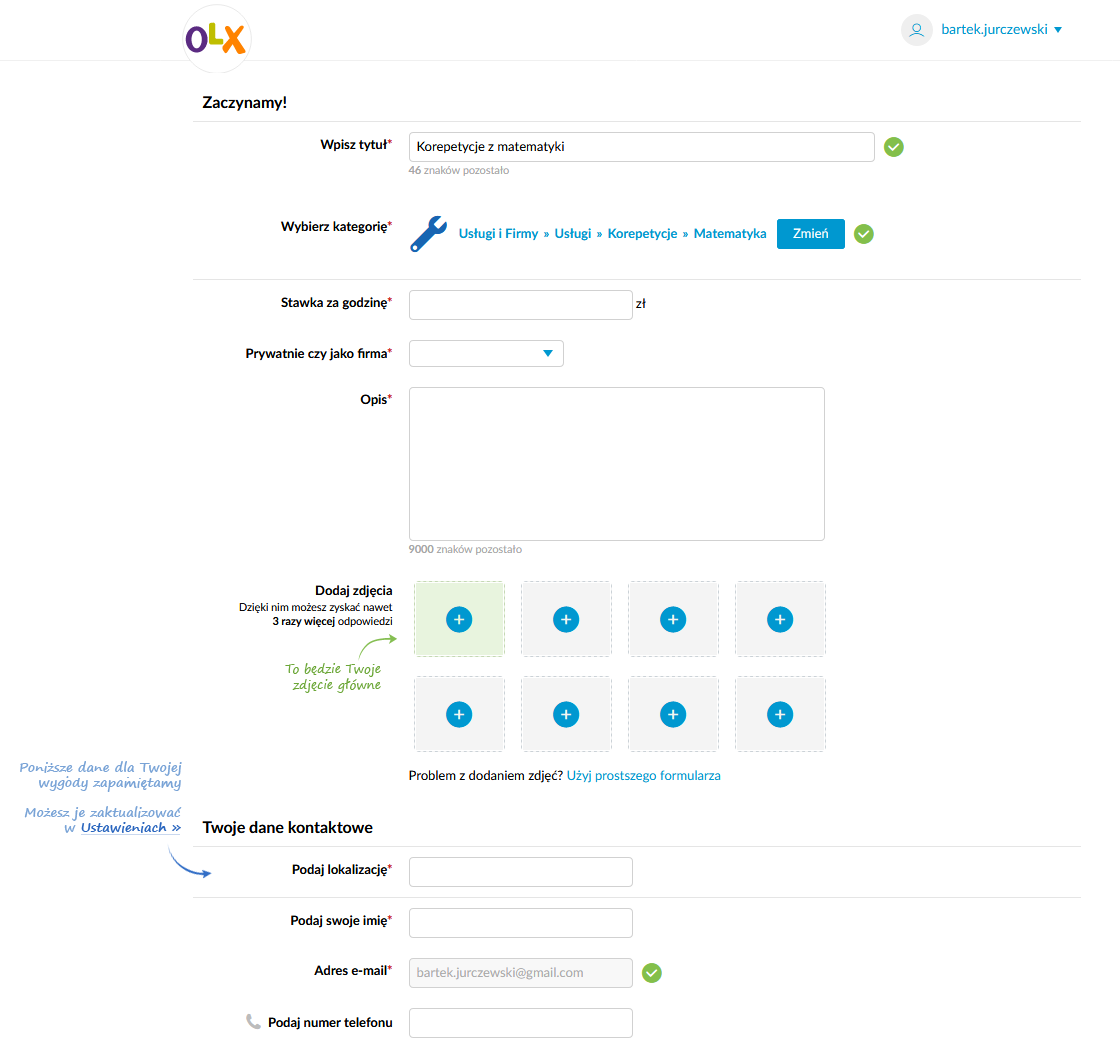
\includegraphics[width=0.95\textwidth]{images/chapter_2/olx-add-announcement.png}
    	\caption{Dodawanie ogłoszenia na serwisie OLX}
    	\label{fig:olx-add-announcement}
    \end{figure}

Rysunek \ref{fig:olx-add-announcement} pokazuje panel dodawania nowych ogłoszeń. 
Użytkownik tego serwisu ma do wypełnianie następujące pola:
\begin{itemize}
    \item tytuł ogłoszenia,
    \item kategoria ogłoszenia(w tym przypadku Usługi),
    \item stawka za godzinę,
    \item jakim jest podmiotem gospodarczym,
    \item opis ogłoszenia,
    \item dodanie zdjęć przedmiotu ogłoszenia,
    \item dane kontaktowe (lokalizacja, imię, nazwisko, adres e-mail, numer telefonu).
\end{itemize}

Jedynym polem, które wyróżnia usługę od przedmiotu jest pole "stawka za godzinę". Zgodnie z ideą tego serwisu, użytkownik nie ma możliwości dodania oceny/recenzji po skorzystaniu z jakiejkolwiek usługi, a co za tym idzie porównania wykonawców usług według ocen. Dodatkowo serwis ten, całkowicie odrzuca element płatności internetowych (w przeciwieństwie do eBaya lub Allegro) i opiera się na płatnościach w świecie rzeczywistym. Płatności przelewami między użytkownikami są odradzane przez sam OLX, ale są oczywiście możliwe z teoretycznego punktu widzenia. Nie ma jednak wtedy żadnej gwarancji, że do takiej wymiany dojdzie ani możliwości reklamacji lub zwrotu po przykładowo słabo wykonanej usłudze lub otrzymaniu produktu niezgodnego z opisem. Odpowiedzią rynku i rozwoju technologicznego są płatności przez Internet.

%%%%%%%%%%%%%%%%%%%%%%%%%%%%%%%%%%%%%%%%%%%%%%%%%%%%%%%%%%%%
%% Płatności internetowe i ich bezpieczeństwo
%%%%%%%%%%%%%%%%%%%%%%%%%%%%%%%%%%%%%%%%%%%%%%%%%%%%%%%%%%%%
\subsection{Płatności internetowe i ich bezpieczeństwo} \label{sec:payments}
Rewolucja cyfrowa dotknęła nie tylko rynku usług i produktów, ale także rynku płatności. W samym 2016 roku tylko 16\% kupujących w Polsce opłaciło swoje zakupy gotówką \cite{gotowka}. Liczba rozwiązań płatności internetowych rośnie z każdym rokiem. Aktualnie na rynku jest ich kilka. Każde z nich różni się pod względem komfortu użytkowania, szybkości i bezpieczeństwa. 

%%%%%%%%%%%%%%%%%%%%%%%%%%%%%%%%%%%%%%%%%%%%%%%%%%%%%%%%%%%%
%% Zwykły przelew bankowy
%%%%%%%%%%%%%%%%%%%%%%%%%%%%%%%%%%%%%%%%%%%%%%%%%%%%%%%%%%%%
\subsubsection{Zwykły przelew bankowy}
Przelew bankowy jest najprostszym i najbardziej analogowym rozwiązaniem. Zaraz po złożeniu zamówienia, dostajemy potwierdzenie zakupu wiadomością e-mail wraz z numerem konta sprzedawcy, kwotą zamówienia i tytułem przelewu (który najczęściej jest numerem zamówienia). Na kupującym ciąży zalogowanie się na stronę banku, utworzenie nowego przelewu i co istotne wypełnienie danymi. Oprócz możliwości pomyłki, na przykład przekopiujemy niepełny numer zamówienia, pomijając jeden znak, ryzykiem, o którym musimy pamiętać jest obecność złośliwego oprogramowania na naszym urządzeniu. Przykładem takiego oprogramowania może być głośna sprawa z 2018 roku, w którym to firma \textit{ESET} natrafiła na konia trojańskiego \textit{BackSwap}. Portal \url{www.zaufanatrzeciastrona.pl} opisuje to oprogramowanie następująco: "Do wstrzyknięcia dochodzi w momencie, gdy klient zleca przelew. Złośliwy kod podmienia wtedy numer rachunku, na który ma zostać wysłany przelew ofiary. Na ekranie komputera tego nie widać – zmiana dotyczy informacji, które przeglądarka wysyła do banku. Przestępcy nie atakują wszystkich przelewów – definiują konkretny przedział kwotowy, który ich interesuje. Ostatnio celowali w kwoty między 10 000 a 20 000 PLN." \cite{backswap}.
Takie ataki są niestety ciągle spotykane. Niektóre banki jak na przykład ING Bank Śląski, po skopiowaniu numeru rachunku bankowego usuwają dwie pierwsze cyfry i proszą klienta o uzupełnienie ich. Bank próbuje wymusić podwójne sprawdzenie numeru konta. Efektem ubocznym będzie możliwość pomyłki przy ponownym wprowadzaniu numeru.

Szybkość przelewu jest zależna od godziny wysłania przelewu. Jest to spowodowane godzinami sesji rozliczeniowych w danych bankach. Najczęściej, jeśli przelew zostanie wysłany do południa, dotrze on popołudniu. W przypadku późniejszych przelewów, dotrze do odbiorcy kolejnego dnia roboczego. Wszystkie przelewy wysyłane w święta i weekendy są dostarczone dopiero kolejnego dnia roboczego. Taka płatność opóźnia wysyłkę/realizację usługi, ponieważ zostanie ona wykonana dopiero wtedy, gdy na rachunku pojawią się przelane środki. 

%%%%%%%%%%%%%%%%%%%%%%%%%%%%%%%%%%%%%%%%%%%%%%%%%%%%%%%%%%%%
%% Przelewy pay-by-link
%%%%%%%%%%%%%%%%%%%%%%%%%%%%%%%%%%%%%%%%%%%%%%%%%%%%%%%%%%%%
\subsubsection{Przelewy pay-by-link}
Przelewy pay-by-link to forma płatności, która cieszy się największą popularnością w Polsce \cite{jak-placa-polacy}. Po wykonaniu zakupów, wybieramy opcję przelewu online, a następnie z listy banków, pokazanych na rysunku \ref{fig:pay-by-link} wybieramy ten z którego chcemy dokonać płatności. 

\begin{figure}[!htbp] 
 	\centering
	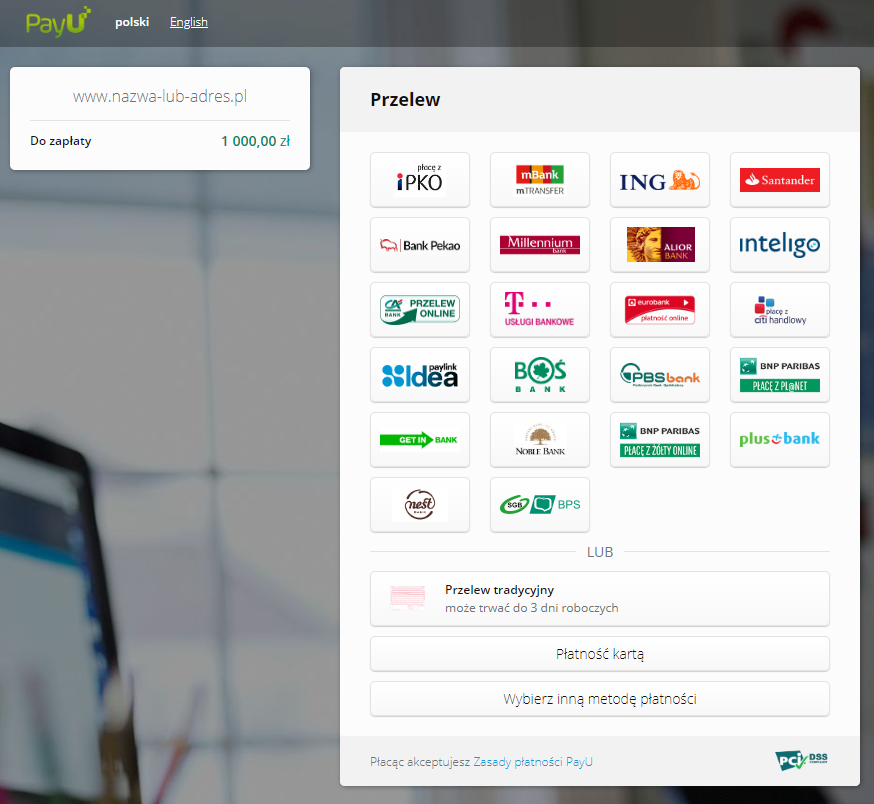
\includegraphics[width=1\textwidth]{images/chapter_2/pay-by-link.png}
	\caption{Przykładowa płatność pay-by-link}
	\label{fig:pay-by-link}
\end{figure}

Po kliknięciu na guzik z logiem banku zostajemy przeniesieni na stronę logowania do danego banku. Po wpisaniu loginu i hasła, pojawi się uzupełniony szablon przelewu, który kupujący musi tylko zatwierdzić. Ostatnim krokiem, kluczowym od strony bezpieczeństwa jest SMS z kodem autoryzacyjnym który otrzymamy. Klient musi przepisać owy kod, aby potwierdzić realizację przelewu. Dzięki temu nawet, jeśli ktoś pozna nasze dane logowania, nie będzie mógł ich użyć do płatności bez posiadania naszego telefonu. Alternatywnym i coraz bardziej popularnym rozwiązaniem jest potwierdzenie przelewu przez aplikację banku. Zanim jednak będzie to możliwe, użytkownik musi się do niej zalogować, co oznacza dodatkowy etap bezpieczeństwa.

Po poprawnym uwierzytelnieniu i potwierdzeniu transakcji, środki trafią niemal natychmiast do sprzedawcy, dzięki czemu od razu będzie on w stanie zrealizować dane zamówienie.

%%%%%%%%%%%%%%%%%%%%%%%%%%%%%%%%%%%%%%%%%%%%%%%%%%%%%%%%%%%%
%% Karta płatnicza
%%%%%%%%%%%%%%%%%%%%%%%%%%%%%%%%%%%%%%%%%%%%%%%%%%%%%%%%%%%%
\subsubsection{Karta płatnicza} \label{sec:cards}
W maju 1998 roku firma \textit{Sequoia Data Corp.} wprowadziła na rynek Compumarket, pierwszy internetowy system e-commerce obsługujący płatności kartą kredytową. Od tego czasu płatności kartą zyskały wiele nowych usprawnień, jednak ich rdzeń pozostał nietknięty. Aby zrealizować płatność, kupujący jest proszony o wpisanie trzech danych: numeru karty, daty jej ważności oraz trzycyfrowego kodu CVC/CVV, znajdującego się na odwrocie karty. Po ich poprawnym zweryfikowaniu, płatność zostaje zakończona. Ta metoda jest tak samo szybka, jak \textit{pay-by-link}, ale mniej wygodna, ponieważ za każdym razem musimy ponownie wpisać dane karty. 

Tradycyjny model płatności zakładał nasze zaufanie do portalu, w którym dokonujemy zakupów, ponieważ osoba posiadająca dane karty mogła samodzielnie dokonać płatności bez naszej zgody. Odpowiedzią na to jest obecna coraz częściej usługa bankowa \textit{3D Secure}. Polega ona na dodatkowym etapie weryfikacji. Po poprawnym wpisaniu danych karty i ich zweryfikowaniu, klient otrzymuje SMSa z kodem weryfikacyjnym. Dopiero po wprowadzeniu go, transakcja jest finalizowana.

Zaletą, która wyróżnia ten rodzaj płatności jest usługa \textit{chargeback}. Portal \url{www.najlepszekonto.pl} opisuje ją następująco: "Chargeback, czyli obciążenie zwrotne, to usługa dostępna tylko dla kart płatniczych. Polega ona na zwrocie środków z konta sprzedawcy, jeśli kupiony przez Ciebie towar nie spełnił Twoich oczekiwań: miał wady, różnił się od tego, co obiecywał sprzedawca, lub w ogóle go nie otrzymałeś. Jeśli próby wymiany towaru w sklepie nie powiodą się, możesz zwrócić się z prośbą o rozstrzygnięcie sprawy przez bank, który jest wystawcą Twojej karty." \cite{chargeback}.

Odmianą fizycznej karty płatniczej jest \textit{karta wirtualna}. Taka karta służy tylko do płatności internetowych. Nie użyjemy jej na przykład podczas zakupów w sklepie stacjonarnym. Po jej wyrobieniu, bank nie przesyła nam jej pocztą, a jedynie podaje nam ich dane, czyli numer, datę ważności i kod CVC/CVV. Niewątpliwą zaletą jest bezpieczeństwo -- nie padniemy ofiarą \textit{skimmingu} (nielegalne skopiowanie zawartości paska magnetycznego w celu utworzenia kopii). Główną wadą takie rozwiązania jest dostępność w Polsce. Aktualnie tylko dwa banki udostępniają taką usługę i to za miesięczną opłatą. 

Zagranicznymi serwisami, które  proponują utworzenie \textit{kart wirtualnych}, jest np. amerykański \url{www.privacy.com}. Portal ten pozwala na proste i nielimitowane tworzenie kart wirtualnych, jak możemy przeczytać na stronie firmy, "jednym kliknięciem". Klient ma możliwość tworzenia karty per portal, czyli na przykład jedna karta do \textit{Netflixa}, kolejna do opłacenia \textit{Spotify} itd. Dodatkowo można ustawić limit obciążenia dla danej strony, wstrzymać płatność lub całkowicie zablokować niechciane opłaty.

%%%%%%%%%%%%%%%%%%%%%%%%%%%%%%%%%%%%%%%%%%%%%%%%%%%%%%%%%%%%
%% Portfele elektroniczne
%%%%%%%%%%%%%%%%%%%%%%%%%%%%%%%%%%%%%%%%%%%%%%%%%%%%%%%%%%%%
\subsubsection{Portfele elektroniczne}

Hybrydą wymienionych wcześniej rozwiązań są \textit{portfele elektroniczne} zwane również \textit{portfelami cyfrowymi}. Rozwiązanie te charakteryzuje się następującymi funkcjami: 
\begin{itemize}
    \item portfel wirtualny (rozumiany jako pula środków do wykorzystania) wraz z możliwością przelania ich bezpośrednio na rachunek bankowy,
    \item płatność wieloma podpiętymi kartami (kredytowymi i debetowymi), także w innych walutach,
    \item możliwość określenia adresu dostawy klienta i innych informacji ułatwiających sfinalizowanie zamówienia.
\end{itemize}

Kolejnym udogodnieniem płatności jest przechowywanie środków w różnych walutach, dzięki czemu użytkownik nie jest obciążony podwójnym przewalutowaniem.

Niektóre portfele oferują też świadczenie usług bez jakikolwiek "przelanych" środków i potrafią służyć jako zaufany pośrednik płatności. Jeśli tylko mamy podpiętą kartę/karty pod taki portfel, możemy w dowolnym miejscu zapłacić owym portfelem, a należność zostanie pobrana natychmiast z naszej wybranej karty. Dzięki temu nie jesteśmy narażeni na potencjalne wady używania samej karty jako środka płatności, opisanych w sekcji \ref{sec:cards}.

%%%%%%%%%%%%%%%%%%%%%%%%%%%%%%%%%%%%%%%%%%%%%%%%%%%%%%%%%%%%
%% Analiza istniejących płatności i portali dla korepetytorów}
%%%%%%%%%%%%%%%%%%%%%%%%%%%%%%%%%%%%%%%%%%%%%%%%%%%%%%%%%%%%
\subsection{Analiza istniejących płatności i portali dla korepetytorów}
Przez lata rozwiązania na rynku usług jak i płatności ewoluowały, często stając się osobnym bytem, a nie dodatkiem do portalu, jak na początku ich istnienia. Firmy odpowiedzialne za nie, przez lata starały się udoskonalić swój produkt i jak najlepiej go wypromować. Poniższa analiza rozwiązań została podzielona na dwie grupy: płatności (jako rdzeń serwisu usług) i serwisów dla korepetytorów.

%%%%%%%%%%%%%%%%%%%%%%%%%%%%%%%%%%%%%%%%%%%%%%%%%%%%%%%%%%%%
%% Płatności
%%%%%%%%%%%%%%%%%%%%%%%%%%%%%%%%%%%%%%%%%%%%%%%%%%%%%%%%%%%%
\subsubsection{Płatności}
Szukając odpowiedniego rozwiązania do obsługi płatności, zdecydowano mieć na uwadze trzy główne cechy: szybkość (jak szybko środki trafią na konto), wygodę (a w tym szybkość wykonania samej płatności) i bezpieczeństwo (transakcji i procesów około-transakcyjnych). Każde z czterech dostępnych rozwiązań zostało szczegółowo opisane w podrozdziale \ref{sec:payments}, właśnie pod kątem tych trzech cech. Stosując takie kryterium, można uznać portfel elektroniczny jako przodownika w tych trzech kategoriach. Dlatego w dalszym rozważaniu jest on tylko brany pod uwagę.

\begin{table}[H]
    \begin{tabular}{|p{5cm}|c|c|c|}
    \hline
     & \multicolumn{1}{l|}{\textbf{PayPal}} & \multicolumn{1}{l|}{\textbf{Visa Checkout}} & \multicolumn{1}{l|}{\textbf{Masterpass}} \\ \hline
    Język polski & \cmark & \cmark & \cmark \\ \hline
    Przypisanie adresu dostawy do konta & \cmark & \cmark & \cmark \\ \hline
    Uwierzytelnianie wiadomością e-mail & \cmark & \cmark & \xmark \\ \hline
    Używanie kart różnych firm & \cmark & \xmark & \xmark \\ \hline
    Możliwość dwustopniowego uwierzytelniania & \cmark & \xmark & \cmark \\ \hline
    Możliwość przechowywania środków w portfelu & \cmark & \xmark & \xmark \\ \hline
    \end{tabular}
    \caption{Porównanie portfeli elektronicznych}
    \label{tab:portfele}
\end{table}

Zestawienie pokazane w tabeli \ref{tab:portfele} pokazuje, że PayPal wygrywa pod względem dwóch funkcji z Visa Checkout i Masterpass -- kryterium użycia kart różnych firm i możliwość przechowywania środków w portfelu.

Ponadto, VisaCheckout i Masterpass są realizowane jako zamknięte środowiska płatnicze. Po kliknięciu na przycisk oznaczony ich logiem, użytkownik zostaje przeniesiony do realizacji płatności. PayPal zdecydował się na inne rozwiązanie, które daje klientowi możliwość zapłaty kartą (Visa, MasterCard i Amex), polskim portalem Przelewy24 (agreguje płatności pay-by-link i kartą omówione w podrozdziale \ref{sec:payments}) i portfelem cyfrowym PayPal. 

\begin{figure}[H] 
 	\centering
	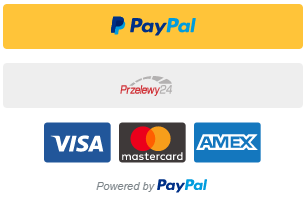
\includegraphics[scale=1.0]{images/chapter_2/paypal-button.png}
	\caption{Smart Payment Button}
	\label{fig:paypal-button}
\end{figure}

PayPal określa swój przycisk jako \textbf{Smart Payment Button} (inteligentny przycisk do płatności), przedstawiony na rysunku \ref{fig:paypal-button}. Oprócz łączenia kilku sposobów płatności, może różnić się on w każdym kraju. Na przykład w Polsce wspiera on portal Przelewy24. Dzięki elastyczności \textit{smart payment button} można być pewnym, że zostanie on dostosowany do kraju, z którego zostaje dokonywane zamówienie, co potencjalnie może zwiększyć zyski ze względu na bogactwo opcji płatności. 

Podsumowując, w grupie portfeli elektronicznych, rozwiązanie PayPal wspiera wszystkie kluczowe i istotne funkcjonalności. Dlatego też, to ono zostało zaimplementowane w aplikacji \textit{Find-A-Tutor} w celu wspierania płatności on-line.

%%%%%%%%%%%%%%%%%%%%%%%%%%%%%%%%%%%%%%%%%%%%%%%%%%%%%%%%%%%%
%% Serwisy dla korepetytorów
%%%%%%%%%%%%%%%%%%%%%%%%%%%%%%%%%%%%%%%%%%%%%%%%%%%%%%%%%%%%
\subsubsection{Serwisy dla korepetytorów}
Na rynku polskim są obecnie dostępne trzy największe serwisy dla korepetytorów. Są to \url{www.e-korepetycje.net}, \url{www.korepetycje.net} i wspomniany już wcześniej portal, nie tylko do korepetycji \url{www.olx.pl}. W tabeli \ref{tab:korepetycje} zestawiono ze sobą cechy tych portali. Cechy zostały pobrane z podrozdziału \ref{sec:problematyka} pokrywającego problematykę pracy.

\begin{table}[H]
    \begin{tabular}{|p{5cm}|c|c|c|c|}
    \hline
     & \multicolumn{1}{l|}{e-korepetycje.net} & \multicolumn{1}{l|}{korepetycje.net} & \multicolumn{1}{l|}{olx.pl} \\ \hline
    Możliwość płatności online & \xmark & \xmark & \xmark \\ \hline
    Ogłoszenia dodawane przez uczniów & \cmark & \xmark & \cmark \\ \hline
    Minimalistyczny design & \cmark & \xmark & \xmark \\ \hline
    Otwarte API & \xmark & \xmark & \xmark \\ \hline
    Aplikacja mobilna & \xmark & \xmark & \cmark \\ \hline
    \end{tabular}
    \caption{Porównanie serwisów dla korepetytorów}
    \label{tab:korepetycje}
\end{table}

Żaden z portali zestawionych powyżej nie obsługuje funkcji tak podstawowej w dzisiejszym świecie, jak płatności elektroniczne. Tylko jeden z nich oferuje przyjazny dla oka i wpisujący się w obecne trendy minimalisty design. Dodatkowo \textit{e-korepetycje.net} i \textit{korepetycje.net} nie posiadają otwartego API, które może posłużyć do stworzenia w przyszłości aplikacji mobilnych. Jednym portalem, który ją dostarcza, jest \textit{OLX.pl}.
\newline
\newline
\textit{Obserwując rynek korepetycji, brakuje na nim rozwiązania które wspiera płatności online. Taką aplikacją jest Find-A-Tutor. Aplikacja serwerowa została stworzona jako otwarte API, dzięki czemu w przyszłości serwis będzie otwarty na powstanie aplikacji mobilnych. Fundamentalną funkcją będzie dodawanie ogłoszeń przez studentów. Ponadto aplikacja kliencka została zrealizowana z minimalistycznym i nieprzytłaczającym designem.}

%%%%%%%%%%%%%%%%%%%%%%%%%%%%%%%%%%%%%%%%%%%%%%%%%%%%%%%%%%%%
%% Techniczne aspekty aplikacji Find-A-Tutor
%%%%%%%%%%%%%%%%%%%%%%%%%%%%%%%%%%%%%%%%%%%%%%%%%%%%%%%%%%%%
\section{Techniczne aspekty aplikacji \textit{Find-A-Tutor}} \label{tech-aspect}
Stworzony projekt składa się z dwóch warstw: 
aplikacji po stronie serwera (backend) i aplikacji po stronie klienta (frontend).
Frontend został napisany w technologii ASP.NET Razor (generujące dynamiczne strony internetowe po stronie serwera) i fundamentalnych technologiach frontendowych, takich jak HTML, CSS, JavaScript i Bootstrap. Wszelkie dane i operacje są wysyłane do backendu przez protokół HTTP, za pośrednictwem JSONa. 
Backend to RESTful WebApi które zostało napisane w najnowszej obecnie wersji aplikacji szkieletowej .NET Core 2.2.

Funkcje rejestracji i logowania do konta zostały napisane przy wykorzystaniu JWT do uwierzytelnienia użytkownika.

Aby zapewnić bezstanowość API, dane są przechowywane w bazie relacyjnej Microsoft SQL Server.

Dla skalowalności rozwiązania wszystkie usługi zostały zamknięte w kontenerach Docker, bazujących na systemie operacyjnym Linux.

%%%%%%%%%%%%%%%%%%%%%%%%%%%%%%%%%%%%%%%%%%%%%%%%%%%%%%%%%%%%
%% Wymagania
%%%%%%%%%%%%%%%%%%%%%%%%%%%%%%%%%%%%%%%%%%%%%%%%%%%%%%%%%%%%
\subsection{Wymagania}
W poniższym podrozdziale opisano wymagania stworzonej aplikacji webowej \textit{Find-A-Tutor}, dzieląc je na funkcjonalne i niefunkcjonalne. 

%%%%%%%%%%%%%%%%%%%%%%%%%%%%%%%%%%%%%%%%%%%%%%%%%%%%%%%%%%%%
%% Wymagania funkcjonalne
%%%%%%%%%%%%%%%%%%%%%%%%%%%%%%%%%%%%%%%%%%%%%%%%%%%%%%%%%%%%
\subsubsection{Wymagania funkcjonalne}
Wymagania funkcjonalne to założenia według, których aplikacja ma się zachować w określony sposób po wystąpieniu danego zdarzenia/zapytania. Wymagania te jasno określają funkcje, jakie ma mieć aplikacja, problemy jakie ma ona rozwiązywać, a także opisują jej ogólną wizję \cite{funkcjonalne}. \\
\noindent
\textbf{Rejestracja jako uczeń lub korepetytor}\\
\indent
Formularz rejestracji umożliwia rejestrację jako użytkownik z rolą ucznia i nauczyciela. Obie te role posiadają odrębne uprawnienia i funkcje opisane poniżej.

\noindent
\textbf{Logowanie jako uczeń, korepetytor i administrator}\\
\indent  
Dostępne są dwa odrębne panele logowania dla użytkownika (ucznia lub korepetytora). Dodatkowym typem konta jest konto administratora, które ma pełne uprawnienia do działania na systemie. Takie konto nie posiada panelu użytkownika, ale może dokonywać wszelakich operacji opisanych w osobnym punkcie, używając zapytań do API.

\noindent
\textbf{Panel ucznia}\\
\indent
Panel ucznia jest dostępny dla użytkownika zalogowanego jako student. Użytkownik ma dostęp do listy wszystkich dodanych przez siebie ogłoszeń. W panelu widnieją następujące dane: data utworzenia ogłoszenia, data podjęcia ogłoszenia, opis ogłoszenia, data wygaśnięcia ogłoszenia, nazwa przedmiotu, status płatności i status ogłoszenia.

\noindent
\textbf{Podgląd szczegółów ogłoszenia}\\
\indent
Panel ucznia umożliwia widok szczegółowy ogłoszenia, który pokazuje informacje dodatkowe takie jak: czas trwania lekcji, cenę za godzinę i całkowitą kwotę do zapłaty. 

\noindent
\textbf{Dodawanie ogłoszeń}\\
\indent
Ogłoszenia mogą być dodawane przez ucznia. Użytkownik wypełnia formularz zawierający następujące dane: opis ogłoszenia, data przedawnienia ogłoszenia oraz przedmiot (wybrany z listy przedmiotów). 

\noindent
\textbf{Płatności online za lekcje}\\
\indent
Po podjęciu ogłoszenia przez korepetytora uczeń ma możliwość opłacenia online należności za ogłoszenie. Po opłaceniu następuje zmiana statusu płatności. 

\noindent
\textbf{Finalizacja ogłoszenia}\\
\indent
Po odbytej lekcji, użytkownik zaznacza zakończenie takiej lekcji, tym samym zmieniając jej status.

\noindent
\textbf{Panel korepetytora}\\
\indent
Użytkownik z rolą nauczyciela ma dostęp do panelu korepetytora. W panelu widnieją wszystkie dostępne ogłoszenia i wszystkie zrealizowane ogłoszenia przez zalogowanego nauczyciela. Panel korepetytora zawiera następujące informacje: data utworzenia ogłoszenia, data podjęcia ogłoszenia, opis ogłoszenia, data wygaśnięcia ogłoszenia, nazwa przedmiotu, status płatności i ogłoszenia.

\noindent
\textbf{Podjęcie ogłoszenia}\\
\indent
Korepetytor ma możliwość podjęcia ogłoszenia z puli dostępnych ogłoszeń. Użytkownik zalogowany jako nauczyciel wprowadza stawkę godzinową wyrażoną w złotówkach. Stawka ta zostaje przypisana do ogłoszenia wraz z kwotą należną za całe ogłoszenie (stawka pomnożona przez liczbę godzin). Po operacji podjęcia, ogłoszenie zmienia status na "podjęte".

\noindent
\textbf{Oddanie ogłoszenia}\\
\indent
Jeśli ogłoszenie, po podjęciu, nie zostało jeszcze opłacone, korepetytor ma możliwość zwrócenia ogłoszenia do ogólnej puli ogłoszeń, tym samym status zmienia się na "niepodjęte".\\

\noindent
\textbf{Konto administratora}\\
\indent
Po zalogowaniu się z rolą administratora, użytkownik może wykonywać operacje CRUD (ang. \textit{create, read, update and delete}) na ogłoszeniach, użytkownikach i liście przedmiotów. Ma możliwość tworzenia, odczytywania, aktualizowania i usuwania rekordów. Użytkownik zalogowany jako administrator może wykonywać wszystkie operacje dostępne dla ucznia czy korepetytora.

%%%%%%%%%%%%%%%%%%%%%%%%%%%%%%%%%%%%%%%%%%%%%%%%%%%%%%%%%%%%
%% Wymagania niefunkcjonalne
%%%%%%%%%%%%%%%%%%%%%%%%%%%%%%%%%%%%%%%%%%%%%%%%%%%%%%%%%%%% 
\subsubsection{Wymagania niefunkcjonalne}

Wymagania niefunkcjonalne określają obszar jakości aplikacji. Wynikają często z wymagań funkcjonalnych lub architektonicznych. Źródłem tych wymagań są przyszli użytkownicy oraz klienci. Do tych wymagań należą skalowalność, kompatybilność, bezpieczeństwo \cite{niefunkcjonalne}.\\
\noindent
\textbf{Przenośność}\\
\indent
Aplikacja powinna być dostosowana do zmiany lokalizacji, środowiska, eksportu danych.

\noindent
\textbf{Skalowalność}\\
\indent
Aplikacja powinna móc się skalowalność pionowo (zwiększenie mocy serwera) i poziomo (zwiększenie instancji aplikacji).

\noindent
\textbf{Otwartość na rozszerzenia}\\
\indent
Aplikacja powinna mieć otwarte API (aplikacje po stronie serwera) i być gotowa na nowe urządzenia, które mogą z niej korzystać (urządzenia mobilne).

\noindent
\textbf{Kompatybilność}\\
\indent
Aplikacja powinna działać w technologiach uniwersalnych i powszechnych dla przeglądarek na silniku Chromium (Chrome, Opera i wkrótce Edge), który na rynku polskim ma 80,65\% udziału w rynku \cite{chrome}.

\noindent
\textbf{Bezpieczeństwo}\\
\indent
Dane użytkowników powinny być poufne i dostępne tylko dla danego użytkownika po zalogowaniu.

\noindent
\textbf{Użyteczność }\\
\indent
Aplikacja powinna być łatwa w obsłudze i powinna zostać zrealizowana z minimalistycznym designem, który nie przytłacza użytkownika.

\noindent
\textbf{Modularność}\\
\indent
Warstwy bazy danych, warstwa graficzna i warstwa  aplikacji (API) powinny być od siebie oddzielone i gotowe do zastąpienia.
    
%%%%%%%%%%%%%%%%%%%%%%%%%%%%%%%%%%%%%%%%%%%%%%%%%%%%%%%%%%%%
%% Narzędzia i technologie użyte w projekcie
%%%%%%%%%%%%%%%%%%%%%%%%%%%%%%%%%%%%%%%%%%%%%%%%%%%%%%%%%%%% 
\subsection{Narzędzia i technologie użyte w projekcie}
Do realizacji aplikacji zostały wybrane tylko te technologie i rozwiązania, które są w pełni darmowe do użytkowania, nawet w projektach komercyjnych, oferują stabilne wersje, które zostały wielokrotnie sprawdzone w setkach innych projektach webowych i są ciągle wspierane i rozwijane do najnowszych standardów. 
%które wyrobiły mocną pozycję w świecie inżynierii oprogramowania. Są to narzędzia dostępne od lat, sprawdzone w wielu aplikacjach i zalecane w projektach webowych. Dodatkowo za cel przyjął sobie takie pojęcia jak czysty kod, czysta architektura oraz korzystanie z jak największej liczby gotowych rozwiązań - tak aby nie rozwiązywać po raz kolejny tych samych problemów.

%%%%%%%%%%%%%%%%%%%%%%%%%%%%%%%%%%%%%%%%%%%%%%%%%%%%%%%%%%%%
%% .NET Core 2.2
%%%%%%%%%%%%%%%%%%%%%%%%%%%%%%%%%%%%%%%%%%%%%%%%%%%%%%%%%%%%    
\subsubsection{.NET Core 2.2}
.NET Core jest darmowym i otwartym \textit{frameworkiem} dla systemów Windows, Linux i macOS. Jest wielo-platformowym następcą .NET Framework. Projekt jest rozwijany przez Microsoft i dystrybuowany na zasadach otwartego oprogramowania (ang. \textit{open source}). Składa się z narzędzi programistycznych, bibliotek oraz środowiska uruchomieniowego \cite{dotnet-core}. 
    
Charakteryzują go następujące cechy:
\begin{itemize}
    \item możliwość programowania i uruchamiania w systemach Windows,\\ macOS i Linux,
    \item zunifikowany scenariusz tworzenia interfejsu API sieci Web i internetowych sieci Web,
    \item system konfiguracji oparty na środowisku, dostosowany do pracy w chmurze,
    \item wbudowane wstrzykiwanie zależności,
    \item lekki, wysoko wydajny modularny potok żądań HTTP,
    \item publicznie dostępny kod i możliwość kontrybucji
    \item obsługa kilku języków programowania: \Csharp, \Fsharp i także Visual Basic,
    \item obsługa menadżera pakietów \textit{NuGet},
    \item elastyczny w wdrożeniu, na przykład poprzez kontereryzacje za pomocą Dockera.
\end{itemize}
%%%%%%%%%%%%%%%%%%%%%%%%%%%%%%%%%%%%%%%%%%%%%%%%%%%%%%%%%%%%
%% C#
%%%%%%%%%%%%%%%%%%%%%%%%%%%%%%%%%%%%%%%%%%%%%%%%%%%%%%%%%%%% 
\subsubsection{C\#}
Jeżyk \Csharp jest językiem obiektowym, opracowanym dla firmy Microsoft, na przełomie tysiąclecia przez zespół pod kierownictwem Andersa Hejlsberga. Jak można przeczytać w oficjalnej dokumentacji języka: 
"Programiści znający którykolwiek z tych języków (C, C++, Java) są zazwyczaj w stanie zacząć produktywnie pracować w \Csharp w bardzo krótkim czasie. Składnia w języku \Csharp upraszcza wiele złożoności C++ i zapewnia zaawansowane funkcje, takie jak typy dopuszczające wartości zerowe, wyliczenia, delegaty, wyrażenia lambda i bezpośredni dostęp do pamięci, których nie można znaleźć w Javie." \cite{csharp} 
    
Podczas opracowywania języka, zespołowi przyświecały następujące założenia projektowe:
\begin{itemize}
    \item obiektowość,
    \item prostota i nowoczesność,
    \item wsparcie dla istniejących zasad inżynierii oprogramowania, takich jak:
    \begin{itemize}
       \item silne typy,
       \item automatyczne czyszczenie śmieci z pamięci (ang. \textit{garbage collector}),
       \item wykrywanie każdej próby odniesienia się do niezainicjowanych zmiennych
    \end{itemize}
\end{itemize}
    
Jako język obiektowy \Csharp obsługuje pojęcia enkapsulacji, dziedziczenia i polimorfizmu. Wszystkie zmienne i metody, w tym metoda \textit{Main} czyli punkt wejścia aplikacji, są zawarte w definicjach klas. Klasa może dziedziczyć bezpośrednio z jednej klasy nadrzędnej, ale może implementować dowolną liczbę interfejsów.

% \subsubsection{Docker}

%%%%%%%%%%%%%%%%%%%%%%%%%%%%%%%%%%%%%%%%%%%%%%%%%%%%%%%%%%%%
%% Kontrola dostępności serwisu
%%%%%%%%%%%%%%%%%%%%%%%%%%%%%%%%%%%%%%%%%%%%%%%%%%%%%%%%%%%% 
\subsubsection{Kontrola dostępności serwisu}
Celem kontroli stanu projektu jest uzyskanie niezależnej oceny, w dowolnym momencie cyklu życia projektu, na temat tego jak dobrze program działa lub czy działa zgodnie z jego założeniami. Skuteczna kontrola stanu (ang. \textit{health check}) zapewnia dostęp do informacji o stanie zależności projektu. Jest to na przykład sprawdzenie czy aplikacja ma połączenie z bazą lub pokazanie w jakiej "kondycji" jest nasz program, na przykład jaki czas zajmuje mu połączenie i wywołanie prostego zapytania do bazy danych.
    
Rozwiązaniem, które dostarcza kontrolę stanów prawie trzydziestu różnych komponentów jest \textbf{AspNetCore.Diagnostics.HealthChecks} \cite{health-checks-github}.
        
\begin{figure}[H] 
    \centering
    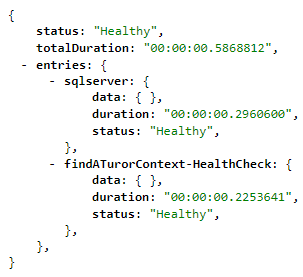
\includegraphics[width=0.5\textwidth]{images/chapter_3/api-health-check.png}
    \caption{Kontrola kondycji aplikacji \textit{Find-A-Tutor}}
    \label{fig:health-check}
\end{figure}
    
Rysunek \ref{fig:health-check} pokazuje stan zależności projektu \textit{Find-A-Tutor (backend)}, wraz z dostępem do bazy danych i czasem który potrzebował na wywołanie zapytania na bazie.

%%%%%%%%%%%%%%%%%%%%%%%%%%%%%%%%%%%%%%%%%%%%%%%%%%%%%%%%%%%%
%% Entity Framework Core
%%%%%%%%%%%%%%%%%%%%%%%%%%%%%%%%%%%%%%%%%%%%%%%%%%%%%%%%%%%% 
\label{EF}
\subsubsection{Entity Framework Core}
\textit{Entity Framework (EF) Core} to rozszerzalny, lekki, otwarty (ang. \textit{open source}) i wielo-platformowy \textit{mapper obiektowo-relacyjny} (ang. \textit{Object-Relational Mapping ORM}). Umożliwia on programistom pracę z bazą danych przy użyciu obiektów .NET. Dodatkowo, w większości eliminuje potrzebę pisania kodu do połączenia się z bazą danych. 
    
Dzięki \textit{EF Core} dostęp do danych odbywa się za pomocą modelu. Model EF przechowuje szczegółowe informacje na temat mapowania klas (wraz z ich polami) na tabele i kolumny bazy danych.
    
\textit{EF Core} obsługuje trzy sposoby realizacji mapowania obiektowo-relacyjnego:
%Model składa się z zmapowanych klas obiektów, zgodnie z ich relacyjnym odpowiednikiem w bazie danych, a także z obiektu kontekstu reprezentującego sesję z bazą danych, która umożliwiając wyszukiwanie i zapisywanie danych.
    
\begin{itemize}
    \item \textit{Code First}: programista określa model obiektów przez kod. Następnie, EF generuje odpowiedni bazodanowy model na podstawie kodu i ustawień konfiguracyjnych dostarczonych przez programistę.
    \item \textit{Database First}: tworzenie modelu obiektów z istniejącej bazy danych.
    \item \textit{Model First}: do stworzenia bazy danych z istniejącego modelu używa się eksportu modelu stworzonego przez \textit{EF}.
\end{itemize}
    
Przykładowy sposób mapowania klasy na struktury bazodanowe, przedstawiono na rysunku \ref{fig:ef}.
    
\begin{figure}[H]
    \centering
    \begin{subfigure}{.6\textwidth}
      \centering
      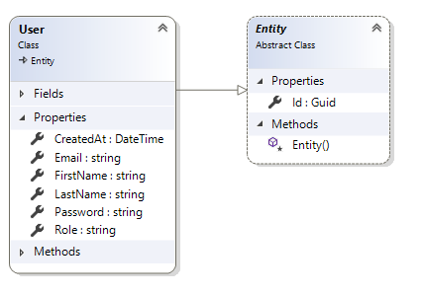
\includegraphics[width=1\linewidth]{images/chapter_3/ef-code.png}
      \caption{Kod klasy \textit{User} (\Csharp)}
      \label{fig:ef-code}
    \end{subfigure}%
    \begin{subfigure}{.4\textwidth}
      \centering
      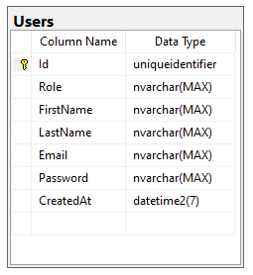
\includegraphics[width=1\linewidth]{images/chapter_3/ef-db.png}
      \caption{Tabela \textit{Users} w bazie danych}
      \label{fig:ef-db}
    \end{subfigure}
    \caption{Mapowanie klas na struktury bazodanowe}
    \label{fig:ef}
\end{figure}
    
Projekt \textit{Find-A-Tutor} został zrealizowany według pierwszego podejścia, czyli \textit{Code First}. Przygotowano domenę, którą następnie za pomocą migracji została odwzorowana na nowo utworzonej bazie danych. 

%%%%%%%%%%%%%%%%%%%%%%%%%%%%%%%%%%%%%%%%%%%%%%%%%%%%%%%%%%%%
%% JWT
%%%%%%%%%%%%%%%%%%%%%%%%%%%%%%%%%%%%%%%%%%%%%%%%%%%%%%%%%%%% 
\subsubsection{JWT}
\textit{JSON Web Token} (w skrócie JWT) to otwarty standard (RFC 7519), który odpowiada za wymianę danych pomiędzy stronami (klient-serwer) w bezpieczny sposób poprzez obiekt w formacie JSON. Informacje przekazywane w nim mogą zostać zweryfikowane przy użyciu cyfrowego podpisu, który jest zawarty w tokenie. Podpis jest generowany za pomocą algorytmu HMAC (\textit{Hash-based Message Authentication Code} czyli kod uwierzytelnienia wiadomości oparty na skrócie) lub klucza publicznego/prywatnego RSA (Rivesta-Shamira-Adlemana) lub ECDSA (\textit{Elliptic Curve Digital Signature Algorithm} czyli algorytm elektronicznego podpisu poprzez kryptografia krzywych eliptycznych).
    
JWT może zostać wykorzystany do:
\begin{itemize}
    \item autoryzacji,
    \item transmisji danych.
\end{itemize}
    
Struktura JWT w swojej wynikowej postaci składa się z trzech części, oddzielonych kropkami. Są to kolejno nagłówek (ang. \textit{header}), zawartość (ang. \textit{payload}) oraz podpis (ang. \textit{signature}). Podział ten jest pokazany na rysunku \ref{fig:jwt}.
    
\begin{figure}[H] 
    \centering
    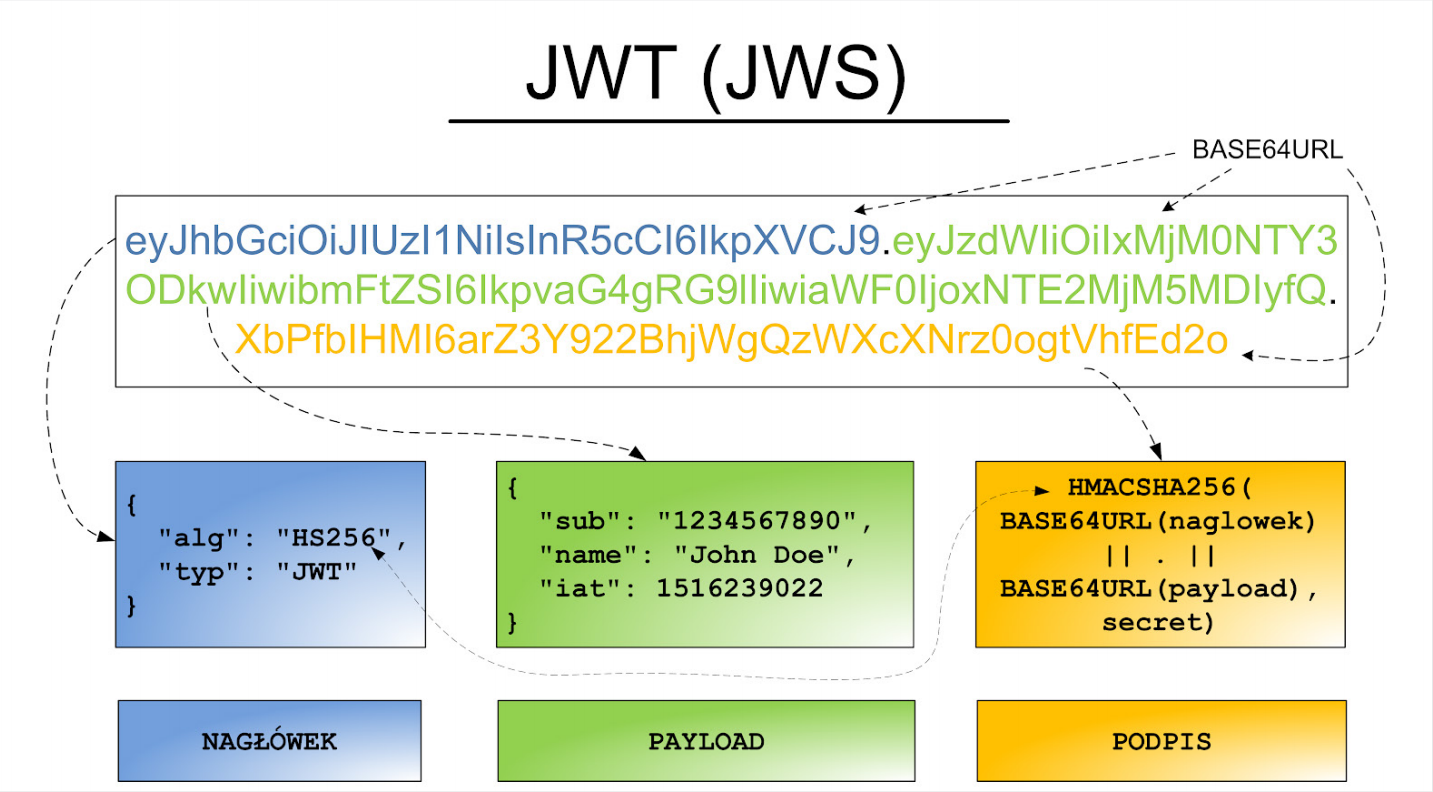
\includegraphics[width=1\textwidth]{images/chapter_3/jwt.png}
    \caption{Przykład podstawowej struktury JWT \cite{sekurak-jwt}}
    \label{fig:jwt}
\end{figure}
    
    \myparagraph{Nagłówek w standardzie JWT}
    \begin{figure}[H] 
     	\centering
    	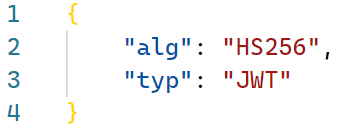
\includegraphics[width=0.35\textwidth]{images/chapter_3/jwt-header.png}
    	\caption{Przykład nagłówka tokenu dla standardu JWT}
    	\label{fig:jwt-header}
    \end{figure}
    
    Nagłówek (pokazany na rysunku \ref{fig:jwt-header}) zawiera dwie informację: rodzaj tokenu na przykład JWT oraz jaki algorytm został użyty do wygenerowania podpisu, na przykład HMAC-SHA256 (zapisywany jako HS256). W postaci końcowej (token), nagłówek jest zapisywany za pomocą algorytmu BASE64URL.
    
    \myparagraph{Zawartość w standardzie JWT}
    Środkowa cześć zawartości tokenu jest odpowiedzialna za przechowywanie danych, które chcemy zawrzeć w tokenie. Są to \textit{roszczenie} (ang. \textit{claims}). Specyfikacja JWT definiuje siedem zarejestrowanych roszczeń. Roszczenia niestandardowe są wykorzystywane w zależności od przeznaczenia tokena.
    Przykład pokazany na rysunku \ref{fig:jwt-payload} pokazuje \textit{Issued At Time, "iat"} czyli datę wydania roszczenia i roszczenie niestandardowe \textit{loggedInAs}.
    
    Zawartość również jest kodowana za pomocą algorytmu BASE64URL.
    \begin{figure}[H] 
     	\centering
    	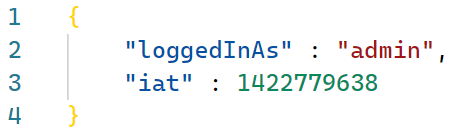
\includegraphics[width=0.5\textwidth]{images/chapter_3/jwt-payload.png}
    	\caption{Przykład zawartości tokenu dla standardu JWT}
    	\label{fig:jwt-payload}
    \end{figure}
    
    \myparagraph{Podpis w standardzie JWT}
    \label{signature}
    
    Podpis cyfrowy potwierdza autentyczność danych zapisanych w tokenie. Walidacja podpisu daje gwarancję, że nadawca wiadomości jest tym, za kogo się podaje.
    
    Podpis haszowany jest za pomocą wybranego algorytmu (w przykładzie na rysunku \ref{fig:jwt-header} jest to HMAC-SHA256). Do tej procedury potrzeba trzech danych: zakodowanego nagłówka za pomocą algorytmu BASE64URL, zakodowanej zawartości za pomocą algorytmu BASE64URL i sekretu. 
    
    \begin{figure}[H] 
     	\centering
    	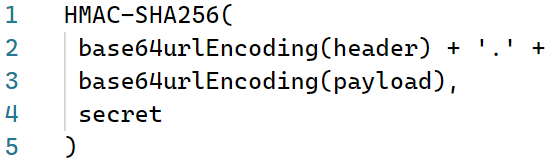
\includegraphics[width=0.55\textwidth]{images/chapter_3/jwt-signature.png}
    	\caption{Sposób obliczania podpisu w standardzie JWT}
    	\label{fig:jwt-signature}
    \end{figure}
    
    \textit{Sekret} to mówiąc najprościej hasło. Serwis autoryzacyjny (w naszym przypadku serwer z API) przechowuje takie hasło i wykorzystuje je przy generowaniu całego tokenu. Hasło musi być tajne, a jego ujawnienie oznacza że każdy może wygenerować taki token i przejść autoryzację w naszym portalu.
    
    \begin{figure}[H] 
     	\centering
    	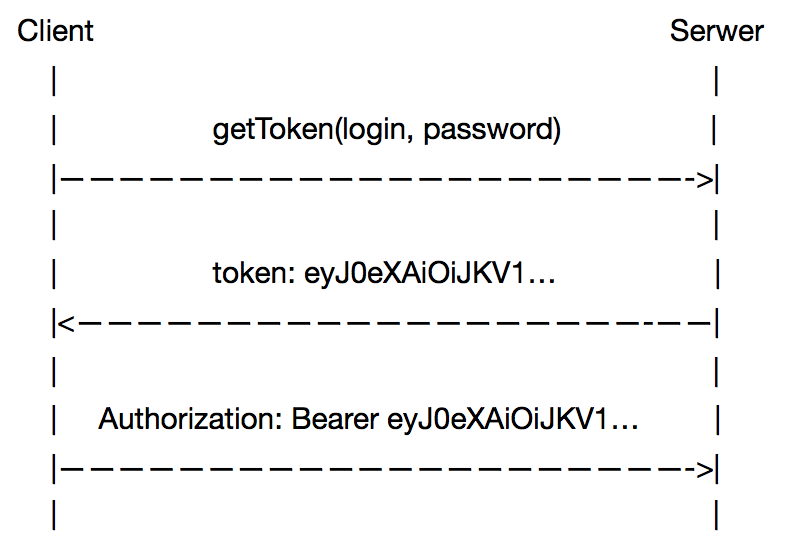
\includegraphics[width=0.8\textwidth]{images/chapter_3/token-diagram.png}
    	\caption{Działanie tokenu w praktyce \cite{token-diagram}}
    	\label{fig:token-diagram}
    \end{figure}
    
    Rysunek \ref{fig:token-diagram} pokazuje proces logowania i wysłania zapytania do API:
    \begin{enumerate}
        \item Logowanie (proces uzyskania tokenu) klient przesyła login i hasło.
        \item Serwer (\textit{Find-A-Tutor.API}) po pomyślnym zweryfikowaniu danych, generuje token JWT, zgodnie z algorytmem opisanym w tej sekcji. Zwraca go jako odpowiedź do poprzedniego zapytania (logowanie).
        \item Użytkownik podczas wysyłania zapytania do API przekazuje także wcześniej otrzymany token. Jeśli token jest poprawny, serwer zwróci odpowiedni dane. Jeśli nie, zwróci komunikat o nieprawidłowym tokenie (lub o jego wygaśnięciu).
    \end{enumerate}
    
%%%%%%%%%%%%%%%%%%%%%%%%%%%%%%%%%%%%%%%%%%%%%%%%%%%%%%%%%%%%
%% Swagger UI
%%%%%%%%%%%%%%%%%%%%%%%%%%%%%%%%%%%%%%%%%%%%%%%%%%%%%%%%%%%% 
\subsubsection{Swagger UI}
\textit{Swagger UI} to otwarty framework wspierany przez duży ekosystem narzędzi, który pomaga programistom projektować, budować, dokumentować i użytkować \textit{WebApi}. 
Swagger UI pozwala na wizualizacje WebApi. Użytkownik ma możliwość zapoznać się ze wszystkimi \textit{endpointami} (adresami), pod które może kierować zapytania. Widzi on, jakie są dostępne kontrolery oraz jakie akcje on udostępnia. Rysunek \ref{fig:swagger} pokazuje akcje dla dwóch kontrolerów (\textit{PrivateLesson} i \textit{SchoolSubject}). 
    
\begin{figure}[!htbp] 
    \centering
    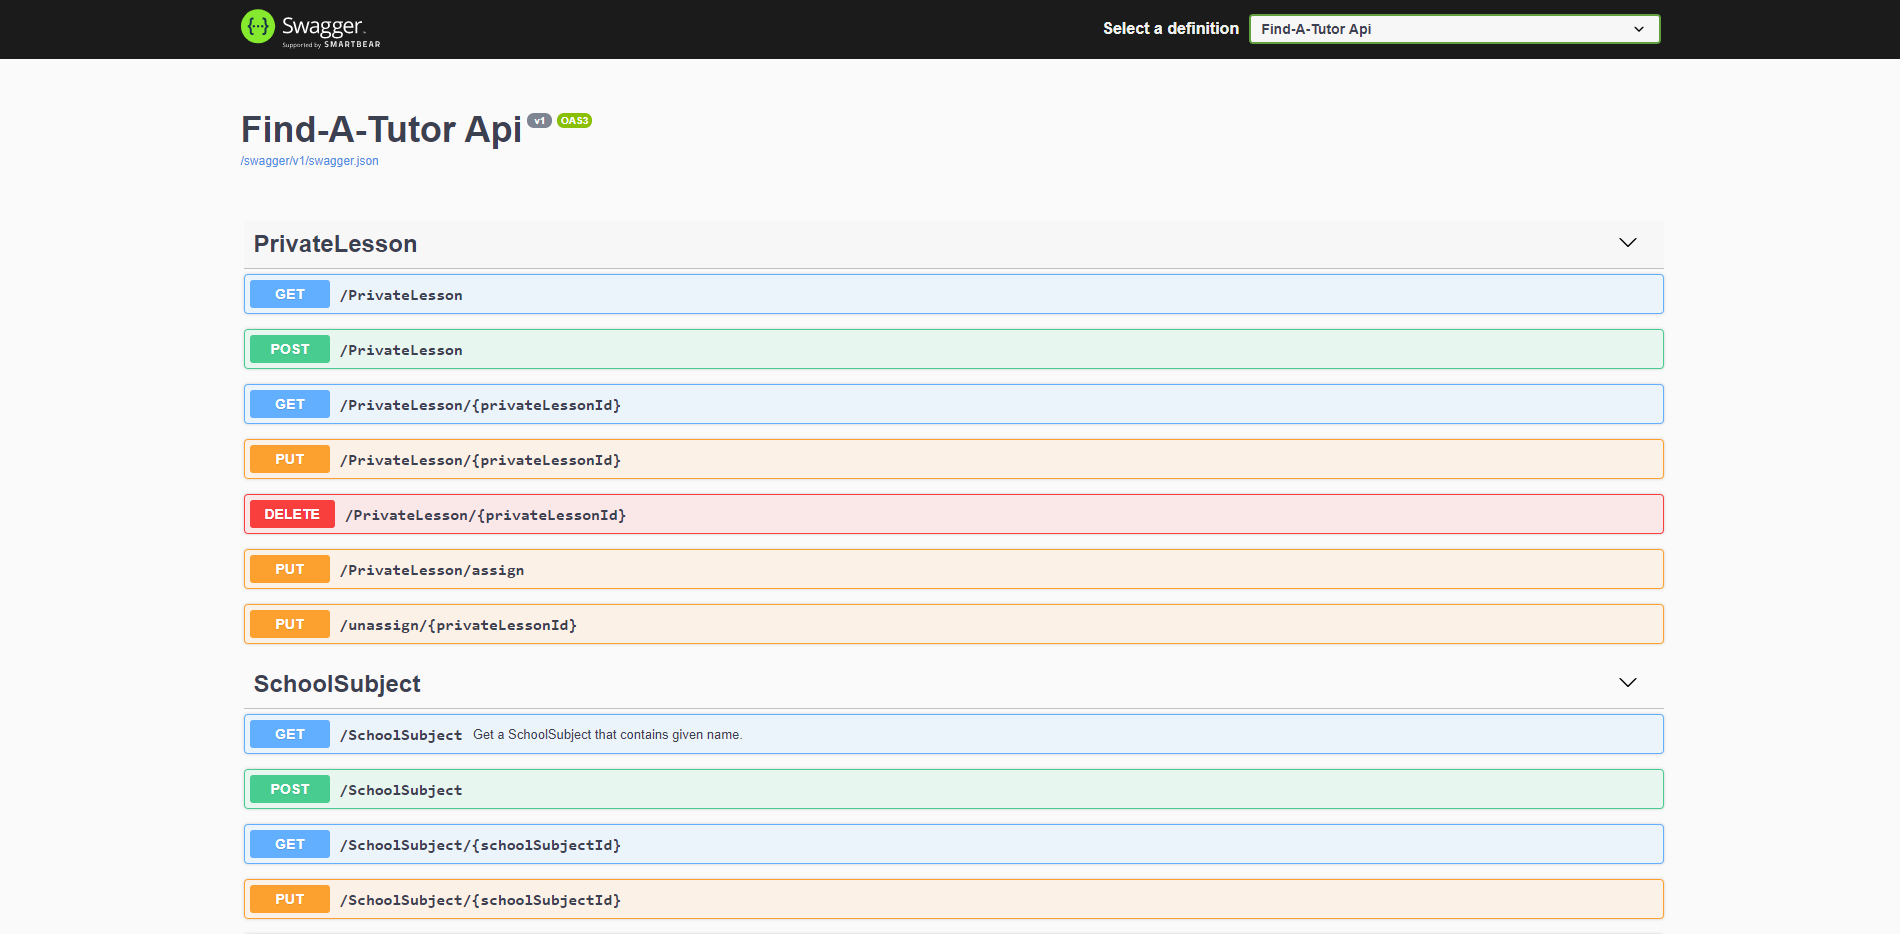
\includegraphics[width=0.9\textwidth]{images/chapter_3/swagger.png}
    \caption{Interfejs Swagger UI dla aplikacji \textit{Find-A-Tutor}}
    \label{fig:swagger}
\end{figure}
    
Dodatkowo, użytkownik ma możliwość przetestowania każdego zapytania, a także zapoznania się z możliwymi odpowiedziami serwera (wraz z modelem), opisem i nazwą argumentów -- na rysunku \ref{fig:swagger-get} jest to zapytanie \textbf{GET} o listę wszystkich przedmiotów szkolnych. 
    
\begin{figure}[!htbp] 
    \centering
    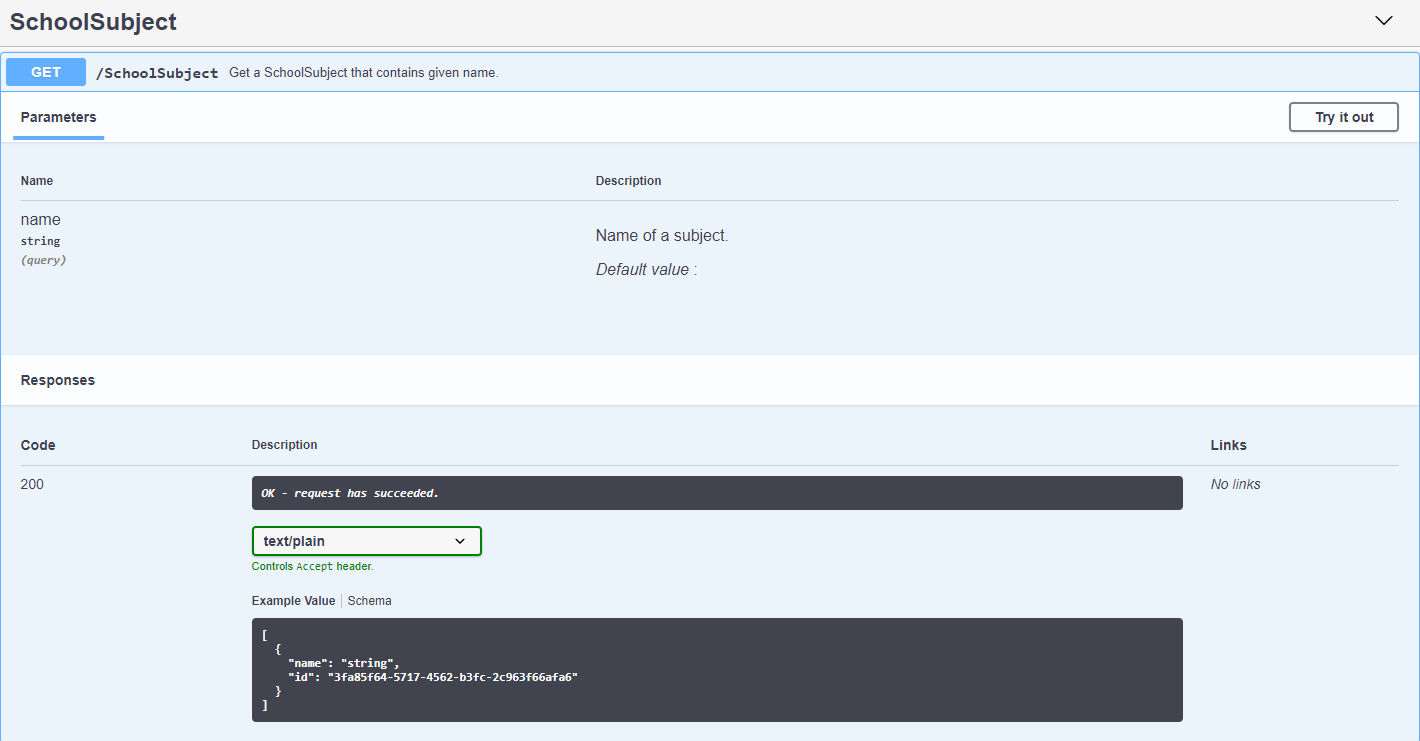
\includegraphics[width=0.9\textwidth]{images/chapter_3/swagger-get.png}
    \caption{Szczegóły zapytania GET}
    \label{fig:swagger-get}
\end{figure}
    
Panel Swagger UI jest dostępny pod adresem /swagger.
% \subsubsection{NLog}
% \subsubsection{Automapper}
% \subsubsection{Figgle}

%%%%%%%%%%%%%%%%%%%%%%%%%%%%%%%%%%%%%%%%%%%%%%%%%%%%%%%%%%%%
%% Architektura aplikacji -- Backend
%%%%%%%%%%%%%%%%%%%%%%%%%%%%%%%%%%%%%%%%%%%%%%%%%%%%%%%%%%%% 
\subsection{Architektura aplikacji -- Backend}
    
Aplikacje, które są zgodne z \textit{Zasadą Odwrócenia Zależności} (ang. \textit{Dependency Inversion Principle}), a także z zasadami projektowania opartego na domenie (ang. \textit{Domain-Driven Design}, DDD) mają tendencję do uzyskiwania podobnej architektury. Ta architektura na przestrzeni lat nosiła wiele nazw. Jedną z pierwszych nazw była \textit{Architektura Heksagonalna} (ang. \textit{Hexagonal Architecture}), następnie \textit{Porty i Adaptery} (ang. \textit{Ports-and-Adapters}). Coraz częściej nazywa się ją \textit{Architekturą Cebulową} (ang. \textit{Onion Architecture}) lub \textit{Czystą Architekturą} (ang. \textit{Clean Architecture}). W niniejszej pracy używa się właśnie tej drugiej nazwy.

\textit{Czysta Architektura} stawia logikę biznesową i model aplikacji w jej środku. Zamiast uzależniania logiki biznesowej od dostępu do danych lub innych problemów związanych z infrastrukturą, zależność ta jest odwrócona: \textit{szczegóły infrastruktury i jej implementacji zależą od rdzenia aplikacji}. Osiąga się to poprzez zdefiniowanie interfejsów lub abstrakcji w rdzeniu aplikacji, które są następnie implementowane przez typy zdefiniowane w warstwie infrastruktury. Każda warstwa jest zależna od warstwy bliżej centrum -- aż do domeny, która nie ma żadnych zależności. Warstwa aplikacji zależy od warstwy domeny, a pozostałe trzy (prezentacji, infrastruktury i utrwalenia) zależy od warstwy aplikacji. Należy podkreślić, że poprawnie wymodelowana domena aplikacji nie posiada żadnych referencji do innych warstw aplikacji.
    
Częstym sposobem wizualizacji tej architektury jest użycie szeregu koncentrycznych kół, podobnych do cebuli. Rysunek \ref{fig:clean-architecture} pokazuje \textit{Czystą Architekturę} przy użyciu tego stylu reprezentacji architektonicznej. Nazwa \textit{Cebulowa Architektura} zawdzięcza nazwę właśnie takiemu ułożeniu warstw.
    
\begin{figure}[H] 
    \centering
    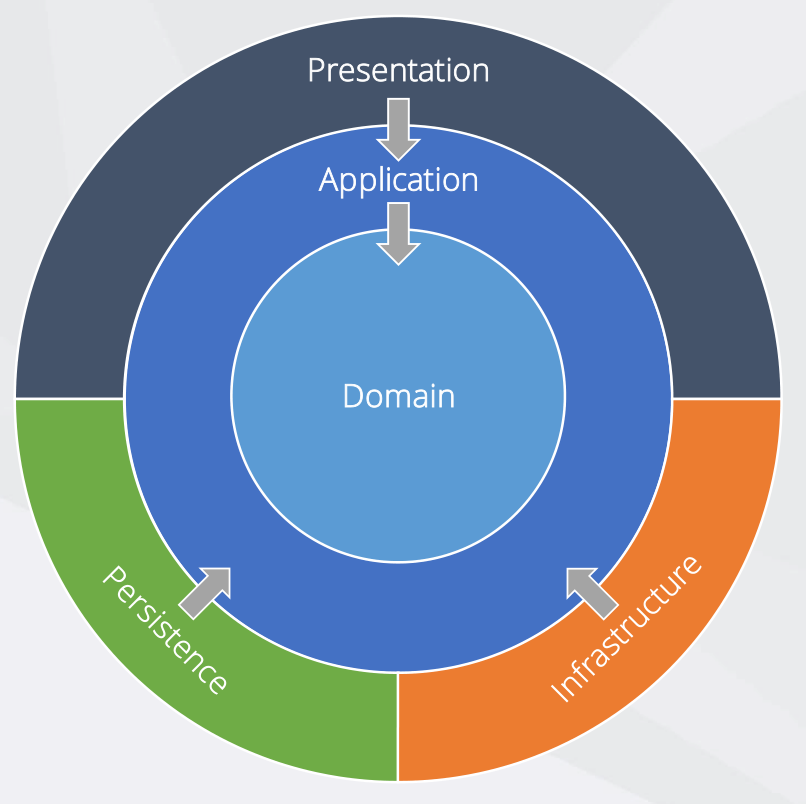
\includegraphics[width=0.7\textwidth]{images/chapter_3/clean-architecture.png}
    \caption{Czysta Architektura \cite{clean-architecture}.}
    \label{fig:clean-architecture}
\end{figure}
    
W projekcie zastosowano właśnie takie rozwiązanie, ze względu na czystość, prostotę implementacji, łatwość zmian (na przykład wymiany infrastruktury na zupełnie nową), a przede wszystkim na czytelność \cite{clean-architecture}. 

    \subsubsection{Rdzeń aplikacji} \label{core}
    Centralnym elementem architektury aplikacji jest \textit{rdzeń} (ang. \textit{core}). Składa się on z \textit{Warstwy domeny} i \textit{Warstwy aplikacji}, pokazanej na rysunku \ref{fig:clean-architecture}. Obie te warstwy zawierają logikę biznesową i logikę aplikacji (wraz ze zdefiniowanymi typami). 
        
    Zgodnie z \textit{PI} (ang. \textit{Persistence Ignorance}) i \textit{Zasadą Ignorowania Infrastruktury} (ang.  \textit{Infrastructure Ignorance}) \textit{rdzeń} musi całkowicie ignorować szczegóły dotyczące trwałości danych (na przykład zapis i odczyt danych). Te zadania powinny zostać wykonane przez warstwę infrastruktury. Dlatego \textit{rdzeń} nie powinien przyjmować bezpośrednich zależności od infrastruktury, co oznacza że ważne jest aby klasy reprezentujące encje modelowe były obiektami \textbf{POCO} (ang. \textit{Plain Old CLR Object}) czyli \textit{zwykłymi starymi obiektami CLR}, gdzie \textit{CLR} to środowisko uruchomieniowe \textit{.Net}. Termin \textbf{POCO} oznacza prosty obiekt, niezawierający logiki biznesowej i nieobciążony dziedziczeniem.
        
    Domenowe encje nie powinny mieć żadnej bezpośredniej zależności (jak dziedziczenie) od frameworka, służącego do dostępu danych, jak na przykład \textit{Entity Framework} (technologia szczegółowo opisana w sekcji \ref{EF}).
        
    %\paragraph{Wzorzec repozytorium}
    \subsubsection{Infrastruktura aplikacji}
    \textit{Warstwa infrastruktury i utrwalenia} (ang. \textit{persistence}) opisuje sposób w jaki dane, które są początkowo trzymane w klasach modelowych (w pamięci) są utrwalane w bazie danych lub w jakiejkolwiek innej postaci. Przykładem takiego utrwalenia jest \textit{Entity Framework Core}. Napisany kod służy do połączanie się z bazą danych przez \textit{DBContext}, który jest reprezentacją bazy danych jako obiektu. Dzięki temu w łatwy sposób można operować na danych w bazie danych.
        
    Ta warstwa zależy od warstw leżących poniżej czyli warstw aplikacji i domeny.
        
    \subsubsection{API aplikacji}
    Warstwą odpowiedzialną za kontakt z otoczeniem aplikacji jest warstwa prezentacji. W projekcie "backendowym", została zaimplementowana jako \textit{WebAPI}, wraz z najpopularniejszym stylem architektury REST. Za format wymiany danych posłużył JSON.
        
        \myparagraph{RESTful WebAPI}
        \indent
        \textit{WebApi} jest to aplikacja, z którą komunikacja jest ograniczona do protokołu HTTP. Protokół ten zawiera 9 metod, przy pomocy których możemy sterować WebAPI. 
        HTTP jest niezależny od platformy i jest bezstanowy - nie zachowuje żadnych informacji o poprzednich transakcjach z klientem. 
        
        Aplikacja taka wystawia na świat adresy URL, zwane \textit{endpointami}.
        Endpointy są rdzeniem aplikacji WebAPI. To właśnie do nich użytkownik końcowy kieruje zapytania. Jako przykładem można posłużyć się następującym endpointem: \textbf{http://domena/privatelesson/3}. Użytkownika interesuje zasób "privatelesson" o ID równym 3. Korzystając z jednej metod protokołu HTTP, czyli GET wysyłamy owe zapytanie.
        
        Gdyby użytkownik skorzystał z metody PUT, mógłby zaktualizować dane znajdujące się pod tym endpointem. Wszystkie metody są opisane przez dokument \textbf{RFC2616} \cite{http}.
        
        REST (ang. \textit{Representational State Transfer}) jest wzorcem architektonicznym, który narzuca dobre praktyki przy tworzeniu aplikacji.
        RESTful WebAPI to WebAPI które stosuje się do zasad wzorca REST i jest zaimplementowane na bazie protokołu HTTP.
        
        \myparagraph{JSON}
        \indent
        \textbf{JavaScript Object Notation} (JSON) to otwarty i lekki format wymiany danych. Charakteryzuje się tekstem czytelnym dla człowieka. Używany jest do przesyłania obiektów danych, składających się z par "atrybut-wartość" i tablicowych typów danych (lub każdej innej wartości możliwej do serializacji) \cite{json}.
        
        Sam zapis jest dokonywany tylko przy użyciu sześciu znaków: \{, \}, [, ], : (dwukropek) oraz , (przecinek). Proces ten został zwizualizowany na rysunku \ref{fig:json}.
        
        \begin{figure}[H] 
         	\centering
        	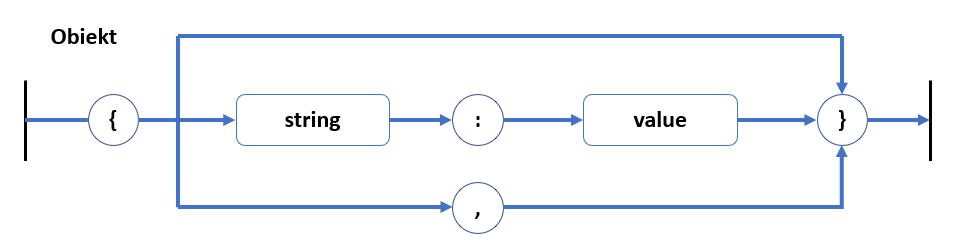
\includegraphics[width=1.0\textwidth]{images/chapter_3/json.png}
        	\caption{Schemat zapisu danych typu \textit{obiekt} w formacie JSON}
        	\label{fig:json}
        \end{figure}
        
        JSON jest niezależny od języka. Wywodzi się on z języka JavaScript, ale prawie wszystkie nowoczesne języki programowania zawierają funkcję generowania i parsowania danych sformatowanych za pomocą JSONa. Dlatego też stał się uniwersalnym formatem do deserializacji danych, przesyłania ich do/z WebAPI, jak i przechowywaniu ich na dysku.
        
        W aplikacji \textit{Find-A-Tutor} stał się on formatem wymiany danych -- WebAPI, przyjmuje i zwraca dane w formacie JSON. 
        
        \begin{figure}[H] 
         	\centering
        	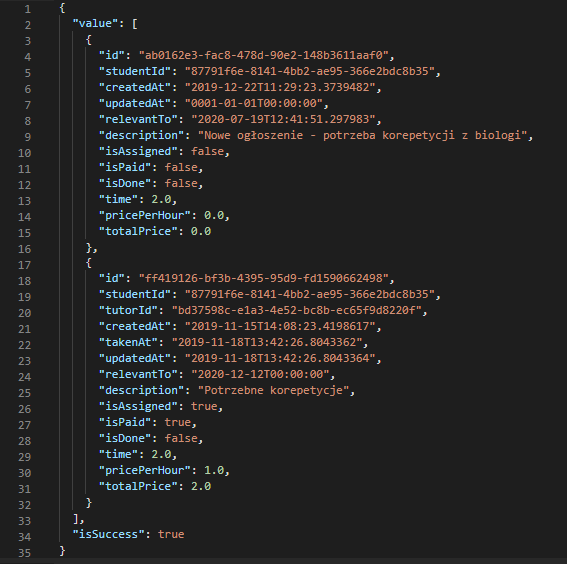
\includegraphics[width=.9\textwidth]{images/chapter_3/json-get.png}
        	\caption{Rezultat wysłanego zapytania do WebAPI}
        	\label{fig:json-get}
        \end{figure}
        
        Na rysunku \ref{fig:json-get} pokazany jest rezultat zapytania metodą GET do WebAPI -- zwracane są wszystkie ogłoszenia danego użytkownika (dodane z jego konta).
        
%%%%%%%%%%%%%%%%%%%%%%%%%%%%%%%%%%%%%%%%%%%%%%%%%%%%%%%%%%%%
%% Architektura aplikacji -- frontend
%%%%%%%%%%%%%%%%%%%%%%%%%%%%%%%%%%%%%%%%%%%%%%%%%%%%%%%%%%%% 
\clearpage
\subsection{Architektura aplikacji -- frontend}
Najmniejsza możliwa liczba projektów dla architektury aplikacji to jeden. W takiej aplikacji, cała logika jest zawarta w jednym projekcie, kompilowana jest do jednego pliku wykonywalnego i wdrożona jako jedna całość. 
    
Ze względu na podział backend -- frontend, to właśnie API (\textit{backend}) odpowiada za faktyczną logikę projektu. I to przez ten interfejs, aplikacja frontendowa porozumiewa się z serwerem lub z bazą danych. 
    
W praktyce każda akcja wykonana na frontendzie (na przykład logowanie, pobieranie danych) odbywa się poprzez wysłanie odpowiedniego zapytania do API. 
    
\subsubsection{MVC}
\textit{Model–view–controller} (\textit{Model-Widok-Kontroler}) to wzorzec architektoniczny powszechnie używany do opracowania aplikacji, posiadających graficzny interfejs użytkownika (Rys. \ref{fig:mvc}). 

\begin{figure}[H] 
    \centering
    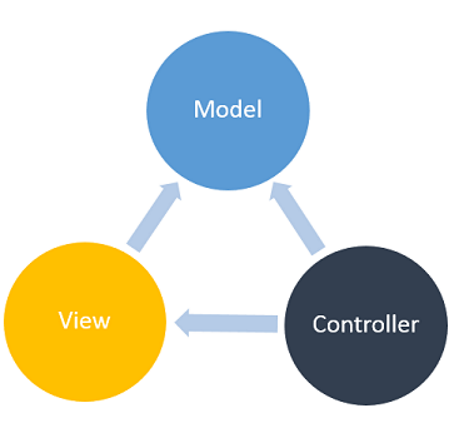
\includegraphics[width=.48\textwidth]{images/chapter_3/mvc.png}
    \caption{Schemat wzorca Model-Widok-Kontroler \cite{mvc}}
    \label{fig:mvc}
\end{figure}
    
MVC dzieli aplikację na trzy części:
\begin{itemize}
    \item Model -- logika biznesowa.
    \item Widok -- graficzny interfejs dla użytkownika.
    \item Kontroler -- obsługuje żądania użytkownika i konwertuje je na polecenia widoku lub modelu.
\end{itemize}
    
Wszystkie części wzorca MVC są ze sobą połączone (Eysunek \ref{fig:mvc}).
Aplikacja frontendowa, projektu \textit{Find-A-Tutor}, została zaprojektowana przy użyciu właśnie tej architektury. 
Prześledźmy zatem pojedynczą akcję użytkownika, na przykład logowanie:
\begin{enumerate}
    \item Użytkownikowi zostaje zwrócony odpowiedni UI (\textit{Widok}).
    \item Użytkownik wpisuje w odpowiednie pola login i hasło .
    \item Aplikacja obsługuje te dane i przekazuje je dalej (\textit{Kontroler}).
    \item Aplikacja opakowuje te dane (JSON) i wysyła jako zapytanie HTTP do WebAPI (\textit{Model}). WebAPI otrzymuje dane i je przetwarza.
    \item WebAPI zwraca dane do aplikacji --są one rozpakowywane i przekazywane dalej (\textit{Model}).
    \item Model aktualizuje Widok, co jest widoczne dla użytkownika.
\end{enumerate}
    
Przepływ danych między częściamy wzorca \textit{MVC} został pokazany na rysunku \ref{fig:mvc-flow}.
    
\begin{figure}[H] 
    \centering
    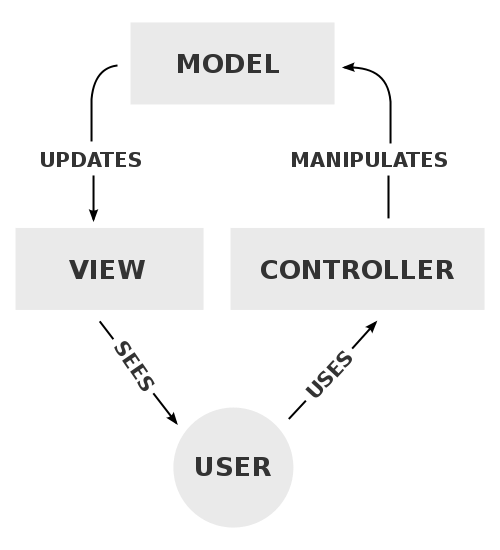
\includegraphics[width=.5\textwidth]{images/chapter_3/mvc-flow.png}
    \caption{Zasada organizacji wzorca projektowego MVC \cite{mvc-flow}}
    \label{fig:mvc-flow}
\end{figure}
    
Przedstawiony scenariusz pokazuje że "frontend" został napisany jako aplikacji klienckiej który obsługuje żądania użytkownika i usprawnia (poprzez UI) komunikacje użytkownika z serwerem. 
Rozdzielenie tych dwóch aplikacji, czyli serwer(\textit{backend) i klient (\textit{frontend}}, ma następujące zalety:
\begin{itemize}
    \item \textit{Modularność} - w razie potrzeby jesteśmy w stanie wymienić jedną z aplikacji na nową.
    \item W razie potrzeby zmiany szaty graficznej aplikacji można w łatwy sposób napisać sam "frontend" od nowa. Dzięki temu cała aplikacja zostaje niezmieniona.
    \item Ułatwienie w utrzymaniu aplikacji i pracy nad projektem.
    \item Możliwość pracy w dwóch osobnych zespołach nad dwoma projektami.
\end{itemize}
    
% \subsubsection{Razor Pages}

%%%%%%%%%%%%%%%%%%%%%%%%%%%%%%%%%%%%%%%%%%%%%%%%%%%%%%%%%%%%
%% Warstwa bazy danych
%%%%%%%%%%%%%%%%%%%%%%%%%%%%%%%%%%%%%%%%%%%%%%%%%%%%%%%%%%%% 
\subsection{Warstwa bazy danych}
Ze względu na charakterystykę aplikacji, zdecydowano się na relacyjną bazę danych.
Zgodnie z wymodelowaną domeną opisaną w sekcji \ref{core} i korzystając z mappera obiektowo-relacyjnego (\textit{EF Core}) opisanego w sekcji \ref{EF}, struktura bazodanowa została wygenerowana za pomocą migracji. Zastosowano obsługiwany sposób \textit{Code First}, czyli na podstawie kodu, EF wygenerował model bazodanowy.
    
Wybrano \textit{Microsoft SQL Server} jako silnik bazodanowy, mając na uwadze, że silnik i platforma \textit{.Net Core} (wraz z \Csharp) została opracowana przez firmę Microsoft. 
    
Rysunek \ref{fig:db} przedstawia strukturę bazy danych dla aplikacji \textit{Find-A-Tutor}: 
\begin{figure}[H] 
    \centering
    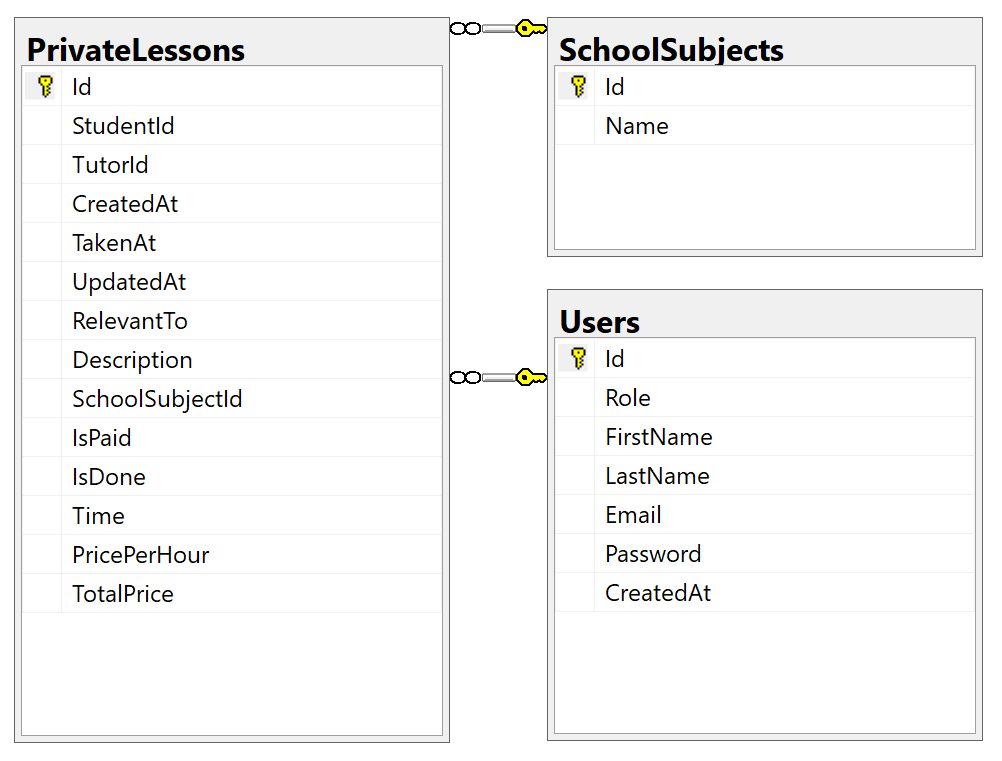
\includegraphics[width=.8\textwidth]{images/chapter_3/db.png}
    \caption{Struktura bazy danych dla aplikacji \textit{Find-A-Tutor}}
    \label{fig:db}
\end{figure}
    
\textit{Podczas powstawania aplikacji Find-A-Tutor starano się aby była ona od samego początku dobrze zaprojektowana tak, by później wszelkie zmiany nie komplikowały nadmiernie stworzonego projektu.}

%%%%%%%%%%%%%%%%%%%%%%%%%%%%%%%%%%%%%%%%%%%%%%%%%%%%%%%%%%%%
%% Aplikacja z punktu widzenia użytkownika
%%%%%%%%%%%%%%%%%%%%%%%%%%%%%%%%%%%%%%%%%%%%%%%%%%%%%%%%%%%%
\newpage
\section{Aplikacja z punktu widzenia użytkownika}
W poniższym rozdziale pokazano działanie aplikacji webowej \textit{Find-A-Tutor}. Zaprezentowane widoki aplikacji zostały wykonane w przeglądarce Chrome w wersji 79. Na rysunku \ref{fig:home} pokazano ekran startowy aplikacji.

\begin{figure}[!htbp] 
    \centering
    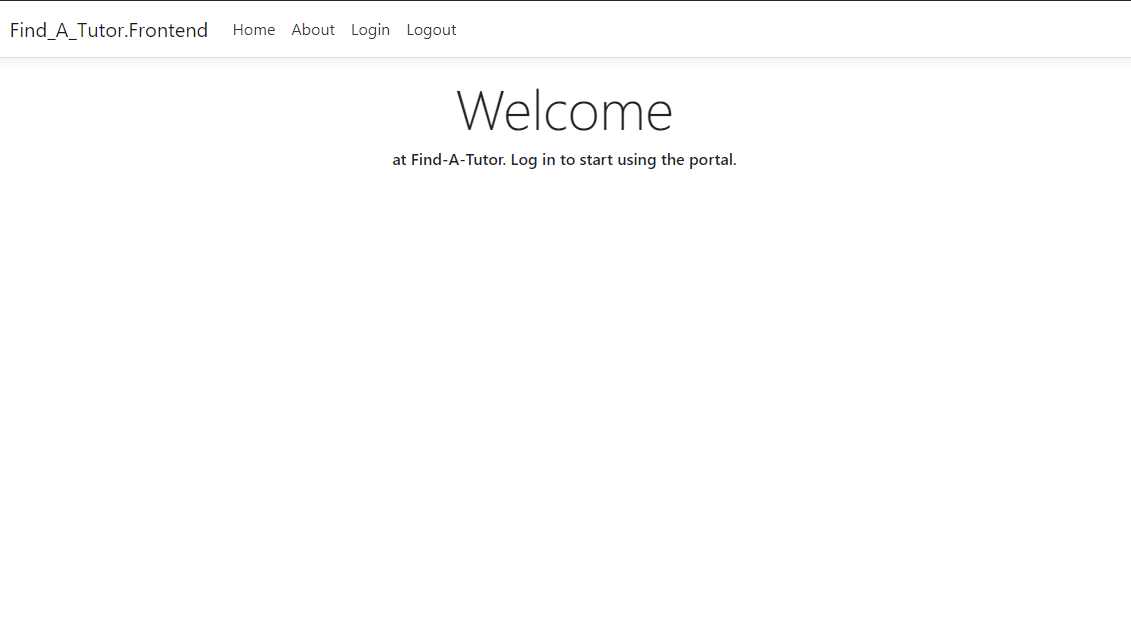
\includegraphics[width=1\textwidth]{images/chapter_4/home.png}
    \caption{Strona startowa aplikacji \textit{Find-A-Tutor}}
    \label{fig:home}
\end{figure}

%%%%%%%%%%%%%%%%%%%%%%%%%%%%%%%%%%%%%%%%%%%%%%%%%%%%%%%%%%%%
%% Uwierzytelnianie
%%%%%%%%%%%%%%%%%%%%%%%%%%%%%%%%%%%%%%%%%%%%%%%%%%%%%%%%%%%%
\subsection{Uwierzytelnianie}
Po kliknięciu na "Login", użytkownikowi ukazuje się panel logowania (Rys. \ref{fig:login}). 

\begin{figure}[!htbp] 
    \centering
    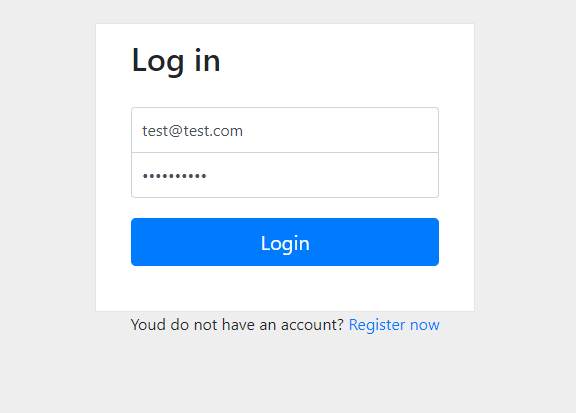
\includegraphics[width=0.7\textwidth]{images/chapter_4/login.png}
    \caption{Panel logowania do panelu użytkownika}
    \label{fig:login}
\end{figure}

Po uzupełnieniu pól (e-mail i hasło) i wciśnięciu przycisku "Login", dane są wysyłane do API. Jeśli uwierzytelnienie się powiedzie, to użytkownik jest przekierowywany do panelu użytkownika.

Jeśli użytkownik nie ma założonego konta, może je założyć za pomocą linku "Register now", który przekierowuje go do podstrony z rejestracją, pokazaną na rysunku \ref{fig:register}.

\begin{figure}[!htbp] 
    \centering
    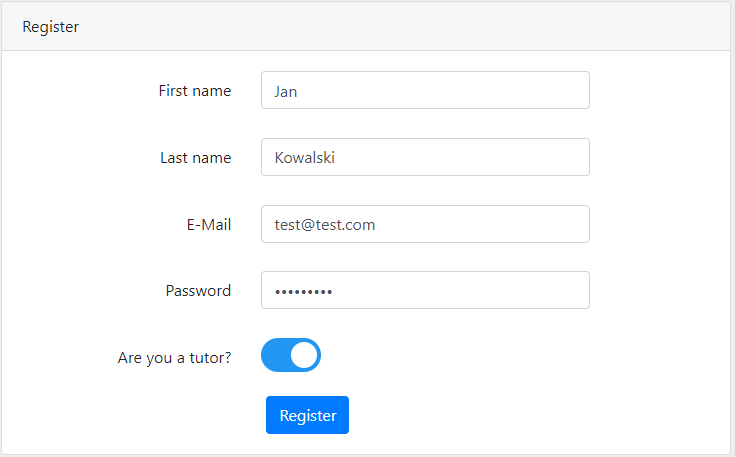
\includegraphics[width=1\textwidth]{images/chapter_4/register.png}
    \caption{Formularz rejestracji}
    \label{fig:register}
\end{figure}

Użytkownik ma do wypełnienia następujące pola: imię, nazwisko, adres email, hasło i typ konta (uczeń lub korepetytor). Poprawność danych sprawdzana jest w locie, dzięki zastosowanym standardom (HTML 5) i po stronie serwera po kliknięciu przycisku "Register".

%%%%%%%%%%%%%%%%%%%%%%%%%%%%%%%%%%%%%%%%%%%%%%%%%%%%%%%%%%%%
%% Panel użytkownika
%%%%%%%%%%%%%%%%%%%%%%%%%%%%%%%%%%%%%%%%%%%%%%%%%%%%%%%%%%%%
\subsection{Panel użytkownika}
W tej sekcji pokazano panel użytkownika i opisano akcje które użytkownik może wykonać za jego pomocą.

\subsubsection{Dodanie nowego ogłoszenia}
Po pomyślnym uwierzytelnieniu użytkownika w roli ucznia, wyświetlany jest panel jego użytkownika (Rys. \ref{fig:student-empty}).

\begin{figure}[!htbp] 
    \centering
    \fcolorbox{black}{black}{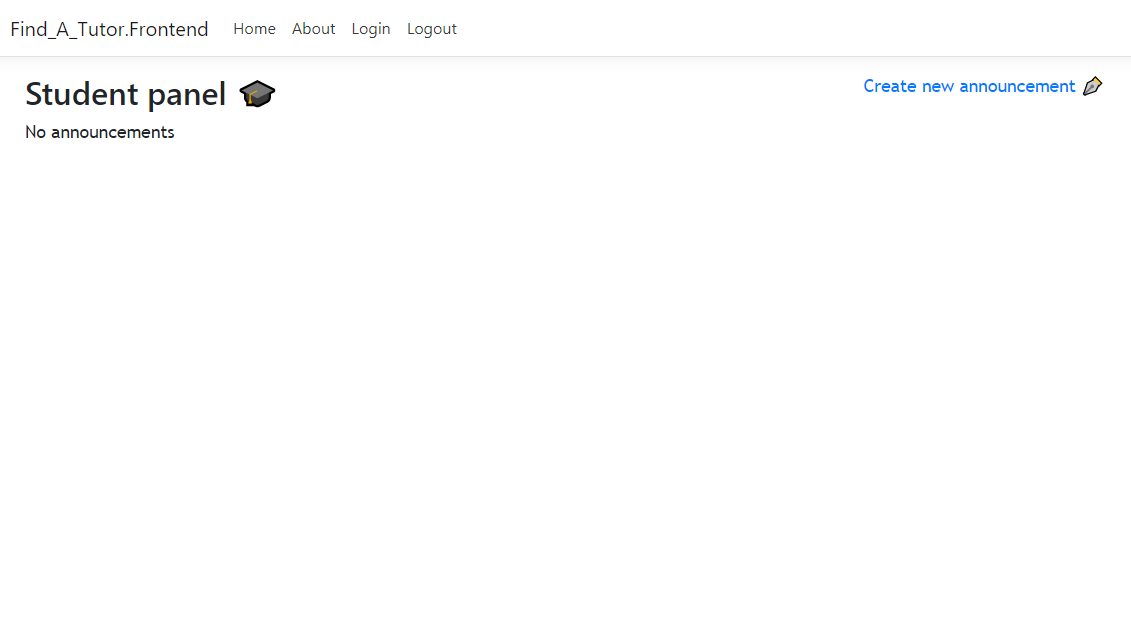
\includegraphics[width=1\textwidth]{images/chapter_4/student-empty.png}}
    \caption{Pusty panel ucznia w aplikacji \textit{Find-A-Tutor}}
    \label{fig:student-empty}
\end{figure}

Panel ten jest pusty. Aby dodać ogłoszenie, klikamy na link "Create new announcement" i zostajemy przekierowani do panelu dodawania nowego ogłoszenia, pokazanego na rysunku \ref{fig:create-new}.
\begin{figure}[!htbp] 
    \centering
    \fcolorbox{black}{black}{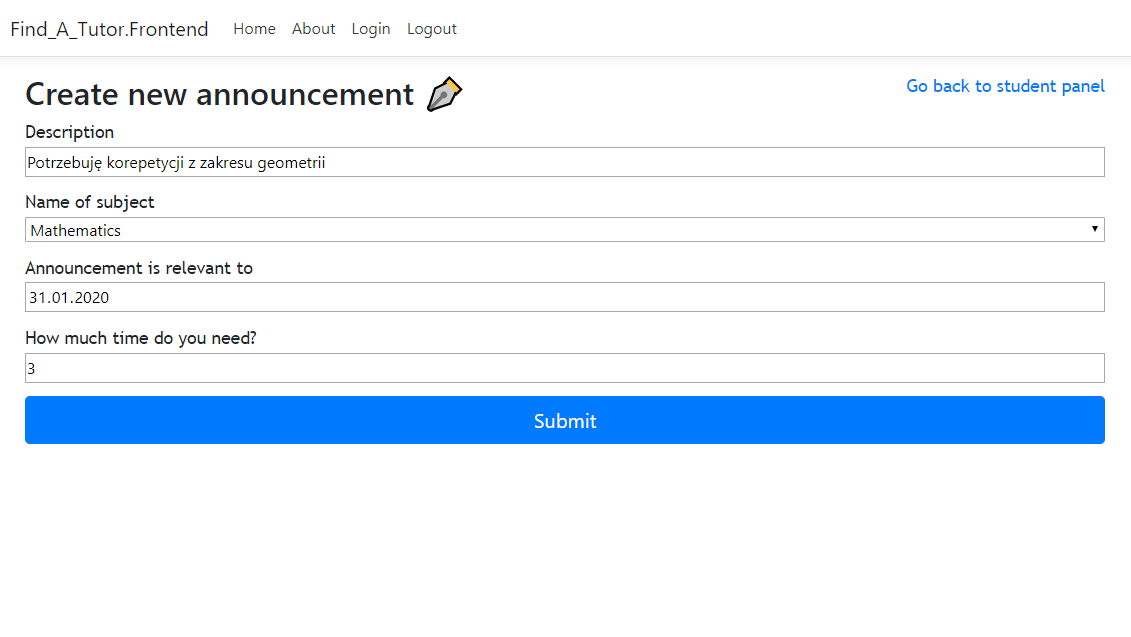
\includegraphics[width=1\textwidth]{images/chapter_4/create-new.png}}
    \caption{Formularz do dodania nowego ogłoszenia w aplikacji \textit{Find-A-Tutor}}
    \label{fig:create-new}
\end{figure}

Użytkownik wprowadza tam następujące informacje: opis, datę ważności ogłoszenia i długość lekcji. Ponadto wybiera przedmiot nauczania z rozwijanej listy. Kiedy dane są wprowadzone, użytkownik klika przycisk "Submit". Następuje wysłanie danych do API. Jeśli wszystko zostanie poprawnie zwalidowane (na przykład data ważności nie jest datą historyczną), użytkownikowi pokaże się komunikat widoczny na rysunku \ref{fig:added}.
\begin{figure}[!htbp] 
    \centering
    \fcolorbox{black}{black}{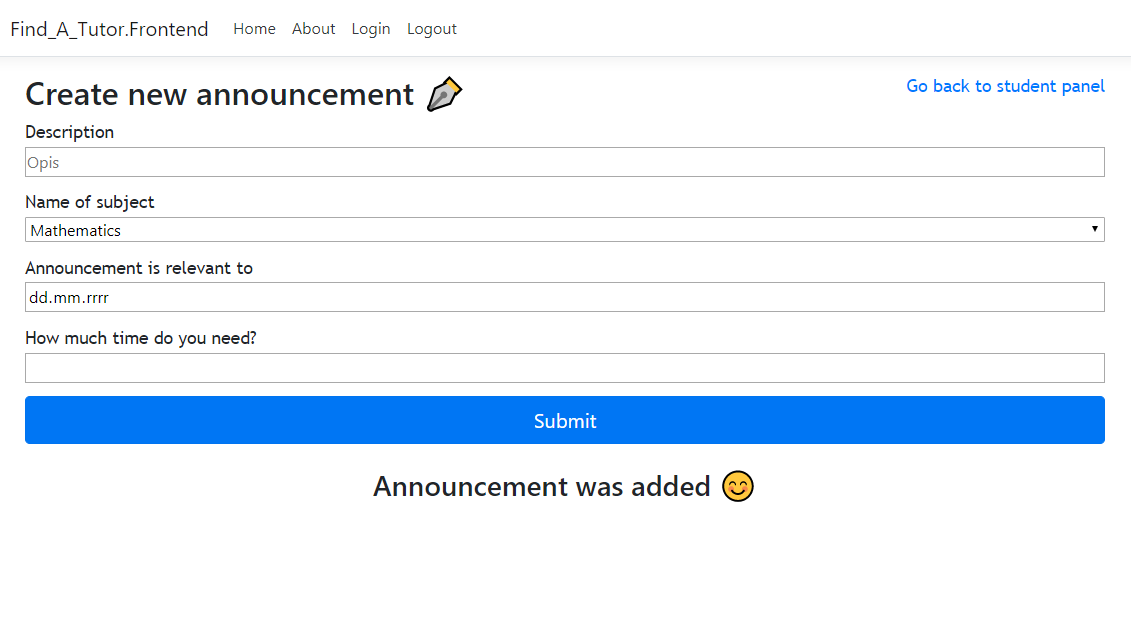
\includegraphics[width=1\textwidth]{images/chapter_4/added.png}}
    \caption{Komunikat po dodaniu nowego ogłoszenia przez ucznia w aplikacji \textit{Find-A-Tutor}}
    \label{fig:added}
\end{figure}

Po powrocie do panelu użytkownika, widoczne jest w nim dodane ogłoszenie (Rys. \ref{fig:student}), wraz z odpowiednimi informacjami o nim: datę utworzenia, datę podjęcia (na razie pusta), datę ważności, przedmiot nauczania, trzy flagi stanu (podjęte, zapłacone i wykonane) i link do podstrony z wszystkimi szczegółami ogłoszenia.
\begin{figure}[!htbp] 
    \centering
    \fcolorbox{black}{black}{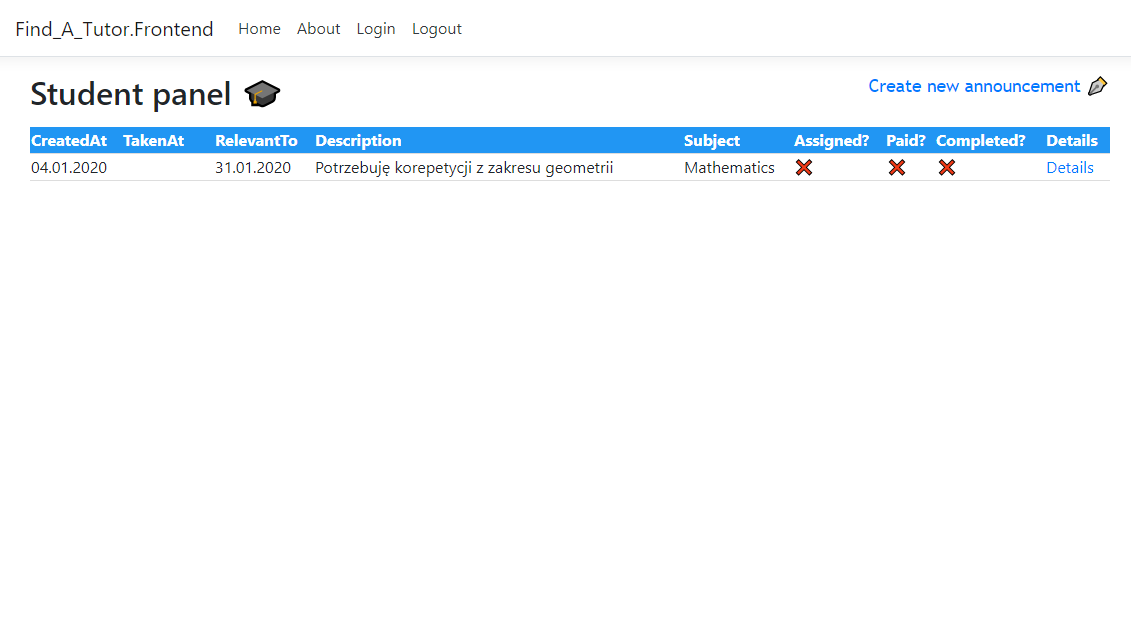
\includegraphics[width=1\textwidth]{images/chapter_4/student.png}}
    \caption{Panel ucznia po dodaniu nowego ogłoszenia w aplikacji \textit{Find-A-Tutor}}
    \label{fig:student}
\end{figure}

%%%%%%%%%%%%%%%%%%%%%%%%%%%%%%%%%%%%%%%%%%%%%%%%%%%%%%%%%%%%
%% Podjęcie ogłoszenia
%%%%%%%%%%%%%%%%%%%%%%%%%%%%%%%%%%%%%%%%%%%%%%%%%%%%%%%%%%%%
\subsubsection{Podjęcie ogłoszenia}
Po pomyślnym uwierzytelnieniu użytkownika w roli nauczyciela, jest wyświetlany panel nauczyciela (Rys. \ref{fig:tutor-empty}).
\begin{figure}[!htbp] 
    \centering
    \fcolorbox{black}{black}{
\includegraphics[width=1\textwidth]{images/chapter_4/tutor-empty.png}}
    \caption{Pusty panel nauczyciela w aplikacji \textit{Find-A-Tutor}}
    \label{fig:tutor-empty}
\end{figure}

Jeśli którykolwiek z uczniów dodał nowe ogłoszenie, to jest ono tutaj wyświetlane (Rys. \ref{fig:tutor}).
\begin{figure}[!htbp] 
    \centering
    \fcolorbox{black}{black}{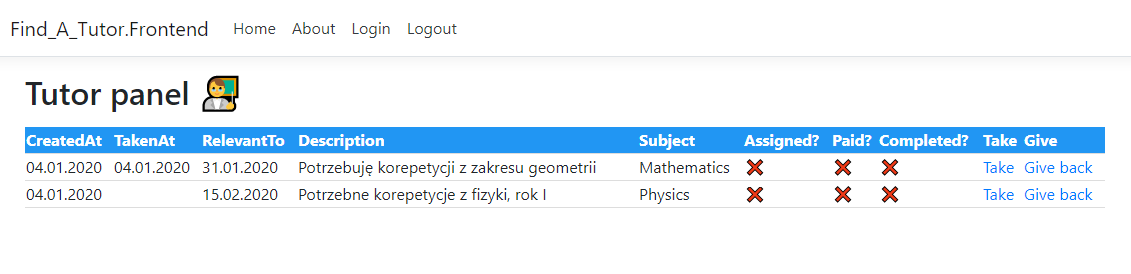
\includegraphics[width=1\textwidth]{images/chapter_4/tutor.png}}
    \caption{Panel nauczyciela w aplikacji \textit{Find-A-Tutor}}
    \label{fig:tutor}
\end{figure}
Użytkownik może wykonać dwie akcje na ogłoszeniu: podjąć je lub oddać je do ogólno dostępnej puli wolnych ogłoszeń. Po naciśnięciu przycisku "Take", użytkownik zostaje przekierowany do podstrony ze szczegółami ogłoszenia (Rys. \ref{fig:take}).

\begin{figure}[!htbp] 
    \centering
    \fcolorbox{black}{black}{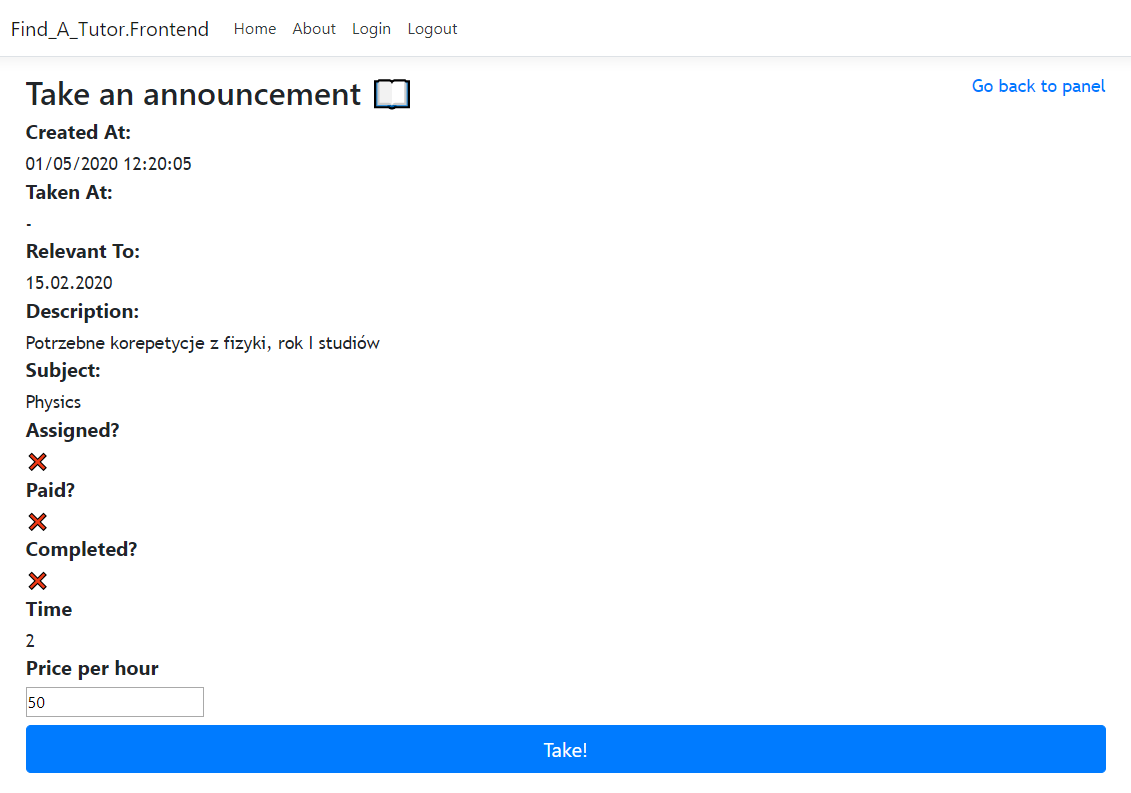
\includegraphics[width=1\textwidth]{images/chapter_4/take.png}}
    \caption{Podjęcie ogłoszenia przez nauczyciela w aplikacji \textit{Find-A-Tutor}}
    \label{fig:take}
\end{figure}

W polu "Price per hour" użytkownik wpisuje stawkę godzinową. Po naciśnięciu przyciska "Take", dana ta jest walidowana, i przesłana do API, a ogłoszenie zostaje przypisane do danego konta nauczyciela.

Podjęcie może nastąpić tylko wtedy, kiedy ono jest wolne. Oddanie ogłoszenia następuje tylko wtedy, kiedy nie jest przypisany do niego nauczyciel i ogłoszenie nie zostało jeszcze opłacone.

Po powrocie do panelu użytkownika, widoczne jest w nim podjęte ogłoszenie wraz z oznaczeniem \cmark w polu "Czy przypisane" (Rys. \ref{fig:tutor-assigned}).
\begin{figure}[!htbp] 
    \centering
    \fcolorbox{black}{black}{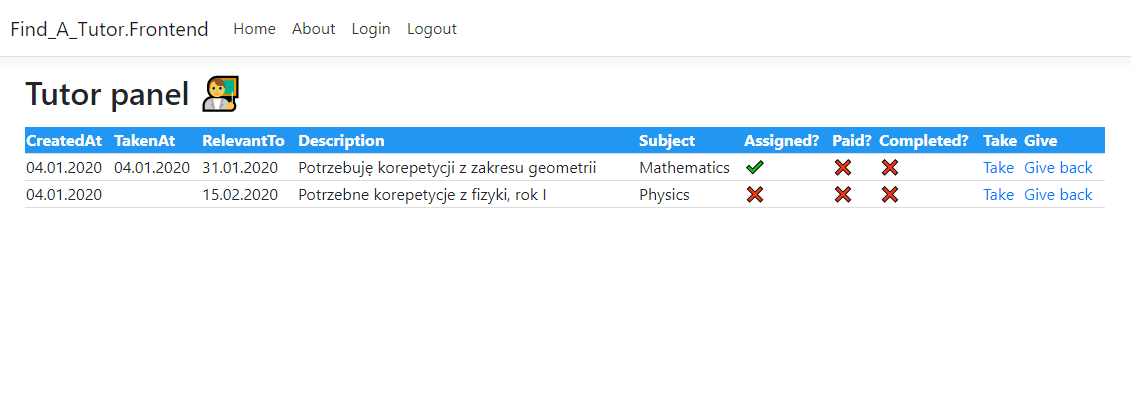
\includegraphics[width=1\textwidth]{images/chapter_4/tutor-assigned.png}}
    \caption{Panel nauczyciela w aplikacji \textit{Find-A-Tutor}}
    \label{fig:tutor-assigned}
\end{figure}

%%%%%%%%%%%%%%%%%%%%%%%%%%%%%%%%%%%%%%%%%%%%%%%%%%%%%%%%%%%%
%% Płatność
%%%%%%%%%%%%%%%%%%%%%%%%%%%%%%%%%%%%%%%%%%%%%%%%%%%%%%%%%%%%
\subsubsection{Płatność}
Po ponownym zalogowaniu w roli ucznia widoczna jest zmiana w ogłoszeniu - zostało ono podjęte (Rysunek \ref{fig:student-assigned}).
\begin{figure}[!htbp] 
    \centering
    \fcolorbox{black}{black}{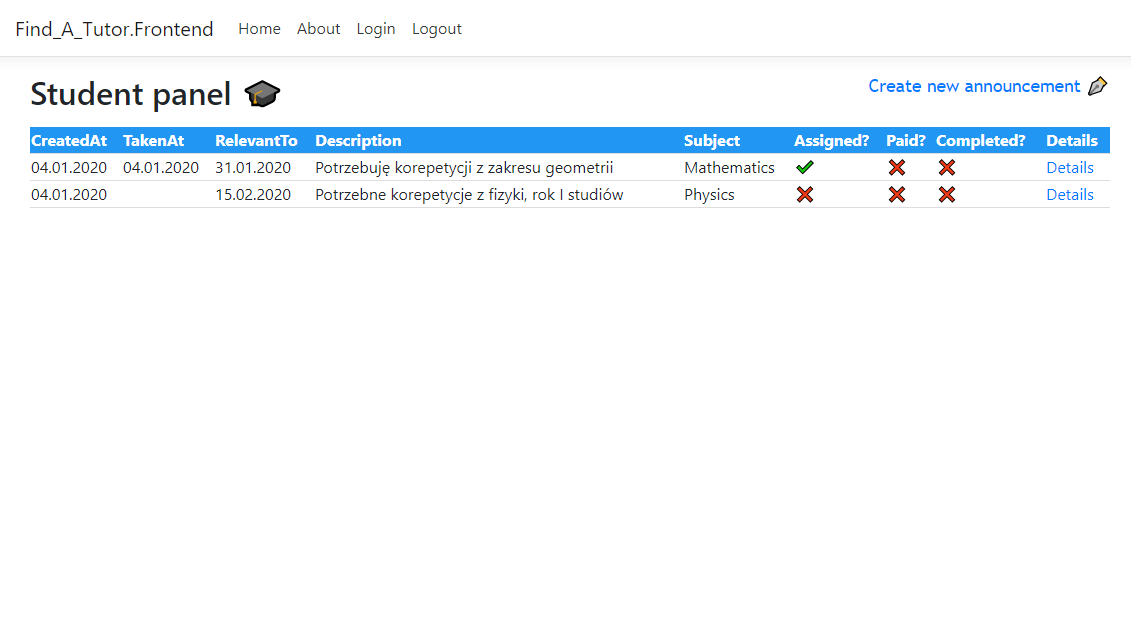
\includegraphics[width=1\textwidth]{images/chapter_4/student-assigned.png}}
    \caption{Panel ucznia w aplikacji \textit{Find-A-Tutor}}
    \label{fig:student-assigned}
\end{figure}

Link "Details" przekierowuje użytkownika do szczegółów ogłoszenia, wraz z możliwością jego opłacenia (Rys. \ref{fig:details}). 
\begin{figure}[!htbp] 
    \centering
    \fcolorbox{black}{black}{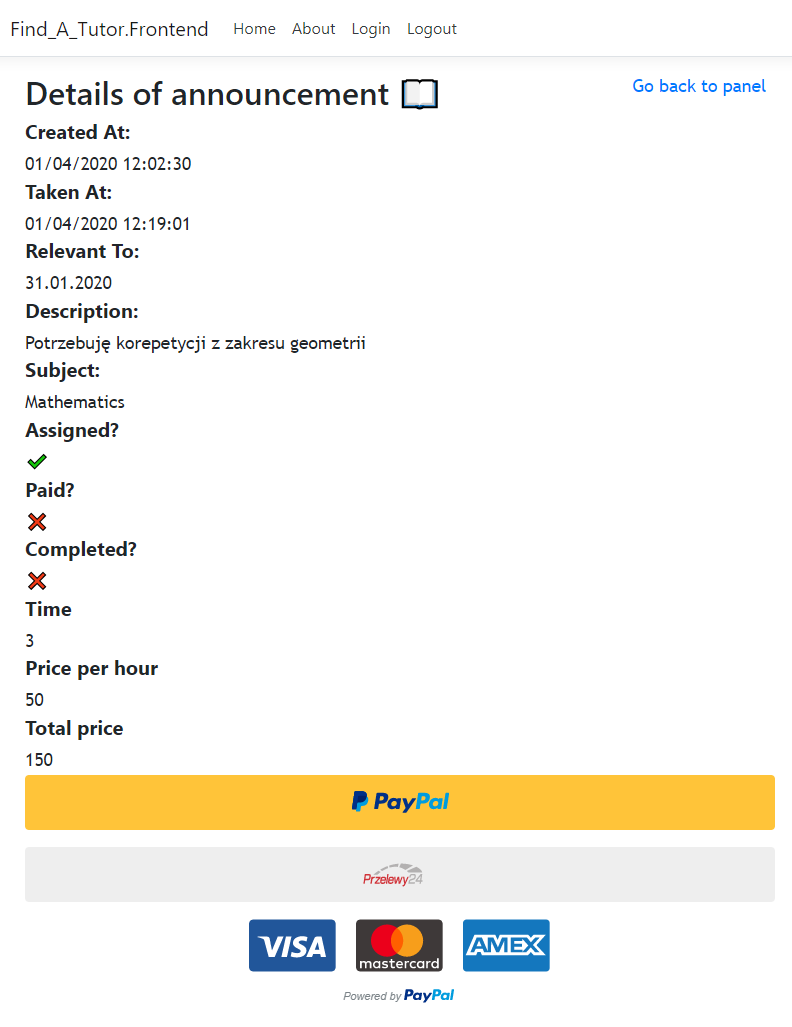
\includegraphics[width=1\textwidth]{images/chapter_4/details.png}}
    \caption{Szczegóły ogłoszenia w aplikacji \textit{Find-A-Tutor} w widoku ucznia}
    \label{fig:details}
\end{figure}

Kwota "Total price" jest wynikiem mnożenia "Time" i "Price per hour". W celu opłacenia, użytkownik wybiera sposób płatności, na przykład przy użyciu portfela elektronicznego PayPal.

\begin{figure}[h]
    \centering
    \begin{subfigure}{.5\textwidth}
      \centering
      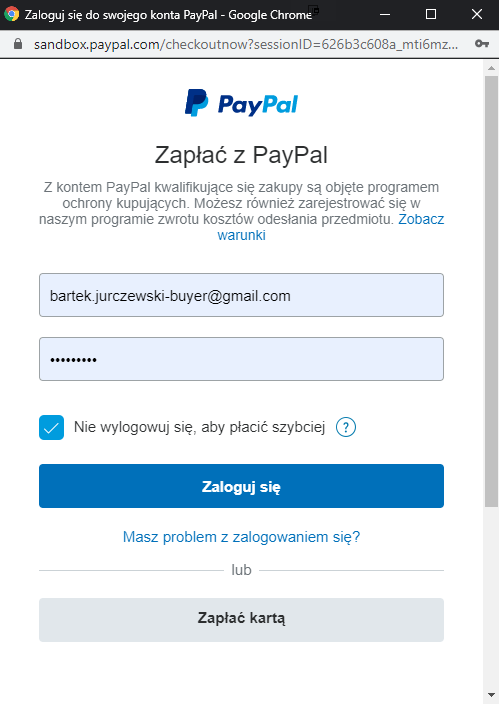
\includegraphics[width=.9\linewidth]{images/chapter_4/pay1.png}
      \caption{Logowanie do serwisu PayPal}
      \label{fig:paypal1}
    \end{subfigure}%
    \begin{subfigure}{.5\textwidth}
      \centering
      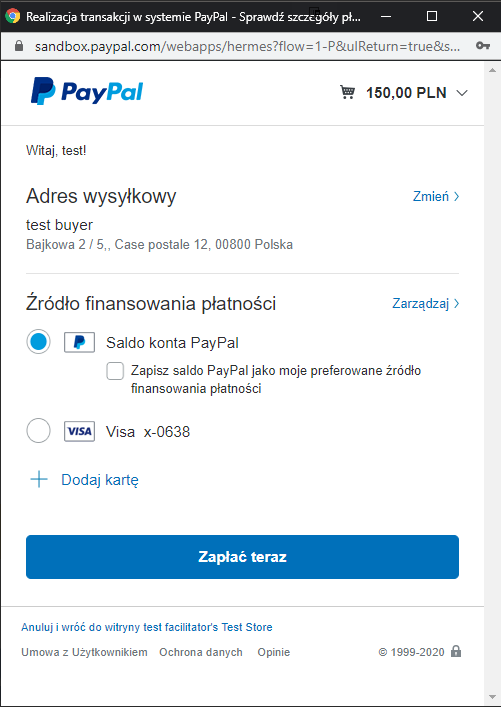
\includegraphics[width=.9\linewidth]{images/chapter_4/pay2.png}
      \caption{Potwierdzenie szczegółów płatności}
      \label{fig:paypal2}
    \end{subfigure}
    \caption{Płatność przy użyciu PayPal}
    \label{fig:paypal}
\end{figure}

Dokonanie płatności zostało pokazane na rysunku \ref{fig:paypal}.

Po przetworzeniu płatności, status ogłoszenia zostaje zaktualizowany. Został on pokazany na rysunku \ref{fig:details-paid}.
\begin{figure}[!htbp] 
    \centering
    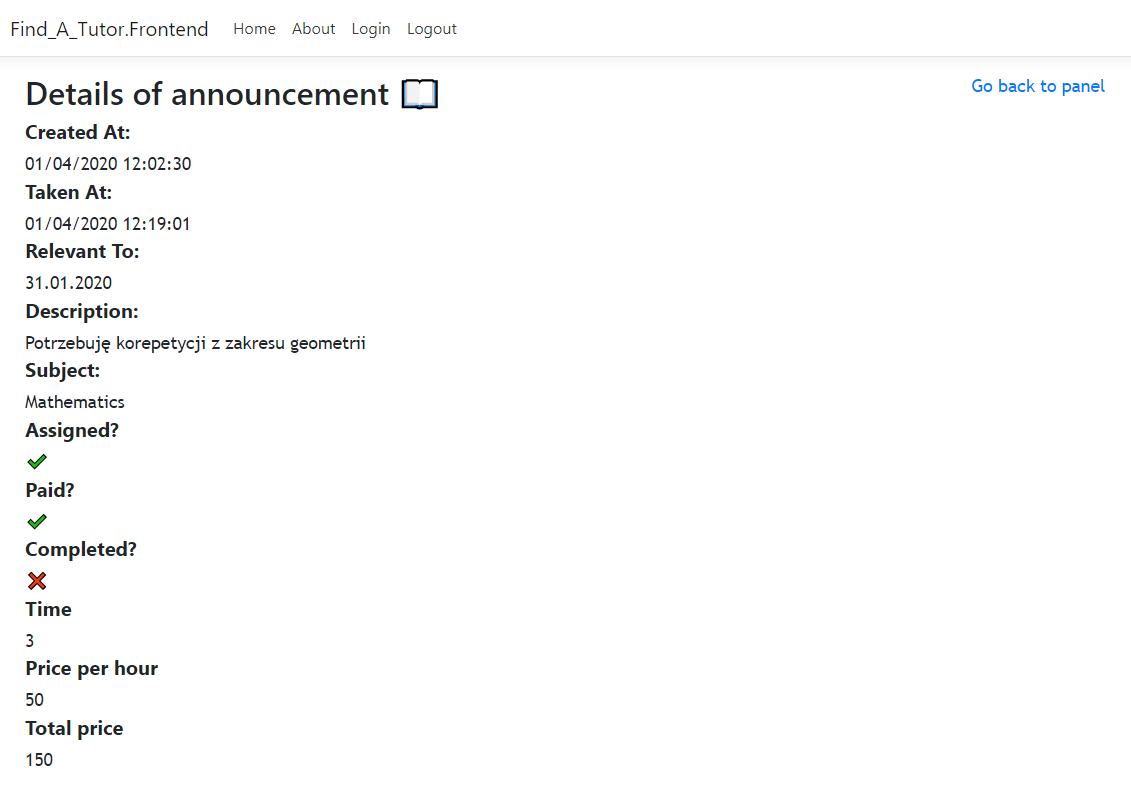
\includegraphics[width=1\textwidth]{images/chapter_4/details-paid.png}
    \caption{Szczegóły zapłaconego ogłoszenia w aplikacji \textit{Find-A-Tutor} w widoku ucznia i studenta}
    \label{fig:details-paid}
\end{figure}

\subsection{Wylogowanie}
Po naciśnięciu przycisku "Logout", na każdej z podstron, następuję zamknięcie sesji i wylogowanie z aplikacji. \newline

\textit{Aplikacja Find-A-Tutor zapewnia wszystkie potrzebne funkcje dostarczając łatwy w obsłudze i wygodny portal do obsługi korepetycji.}

%%%%%%%%%%%%%%%%%%%%%%%%%%%%%%%%%%%%%%%%%%%%%%%%%%%%%%%%%%%%
%% Wnioski
%%%%%%%%%%%%%%%%%%%%%%%%%%%%%%%%%%%%%%%%%%%%%%%%%%%%%%%%%%%%
\pagebreak
\section{Podsumowanie}
Pierwszym etapem niniejszej pracy dyplomowej była analiza dwóch rynków: usług i płatności internetowych. Analiza rynku usług dowiodła, że dostępne rozwiązania, takie jak \url{www.olx.pl}, oferują tylko podstawowe funkcje. Przede wszystkim brakuje w nich płatności cyfrowych (w jakiekolwiek formie). Dodatkowo, pomogła ona dostrzec niszę -- rynek korepetycji, który mimo podstawowego zagospodarowania, popełnia błędy całego rynku usług. W dalszej części pracy została dokonana analiza rynku płatności cyfrowych w celu dostarczenia jak najlepszego systemu dla użytkownika końcowego. W analizie zostały nie tylko porównane obecne rozwiązania (przelewy tradycyjne, pay-by-link, karta płatnicza i portfele elektroniczne), ale także spośród zwycięzcy na tym polu -- portfeli elektronicznych -- zostało przeprowadzone zestawienie obecnych liderów na tym rynku. Zwycięskim rozwiązaniem okazał się PayPal. 

Celem pracy było dostarczenie aplikacji webowej która w łatwy sposób pozwoli na zarządzanie korepetycjami z punktu widzenia ucznia nauczyciela. Rozwiązanie takie zostało wykonane w sposób modularny, zgodnie z \textit{Czystą Architekturą}. Aplikacja jest otwarta na modyfikacje w przyszłośc i na wymianę poszczególnych elementów. Ponadto, struktura aplikacji pozwoli w przyszłości zastosować implementację innych systemów płatności. Wpływa to przede wszystkim na cykl życia aplikacji, która przez kolejne lata może nie być dalej rozwijana, ale same płatności portfelem elektronicznym będą aktualizowane. Od strony frontendowej, aplikacja \textit{Find-A-Tutor} oferuje przejrzysty i czytelny interfejs który ułatwi użytkowanie portalu. 

Zaimplementowany system PayPal, który zwyciężył w analizie rynkowej, jest liderem płatności online. Inne firmy technologiczne, nawet te największe, takie jak Facebook lub Google są ze swoimi rozwiązaniami daleko za PayPalem. Pomimo tego, że implementacja i testy nowych portfeli elektronicznych mogą być gotowe w niedalekiej przyszłości, to dogonienie konkurencji pod względem przekonania do siebie użytkowników i utwierdzenie ich w rewolucyjności ich rozwiązania może zająć lata.

W przyszłości rynek usług będzie z pewnością ewoluował wchłaniając kolejne gałęzie przemysłu. Będzie to oznaczało zwiększenie agregatów ogłoszeń (na przykład \url{www.olx.pl}) i powstanie zupełnie nowych aplikacji, takich jak \textit{Find-A-Tutor}. Zaproponowana aplikacja może stanowić ciekawe rozwiązanie dla osób próbujących stworzyć autorską implementację serwisu ogłoszeniowego.

    \clearpage

%%%%%%%%%%%%%%%%%%%%%%%%%%%%%%%%%%%%%%%%%%%%%%%%%%%%%%%%%%%%
%% Indeks rysunków
%%%%%%%%%%%%%%%%%%%%%%%%%%%%%%%%%%%%%%%%%%%%%%%%%%%%%%%%%%%%     
    \section{Indeks rysunków}
        \listoffigures
    \clearpage    
    
%%%%%%%%%%%%%%%%%%%%%%%%%%%%%%%%%%%%%%%%%%%%%%%%%%%%%%%%%%%%
%% Indeks tabel
%%%%%%%%%%%%%%%%%%%%%%%%%%%%%%%%%%%%%%%%%%%%%%%%%%%%%%%%%%%% 
    \section{Indeks tabel}
        \listoftables
    \clearpage
    
%%%%%%%%%%%%%%%%%%%%%%%%%%%%%%%%%%%%%%%%%%%%%%%%%%%%%%%%%%%%
%% Bibliografia
%%%%%%%%%%%%%%%%%%%%%%%%%%%%%%%%%%%%%%%%%%%%%%%%%%%%%%%%%%%%     
    \section{Bibliografia}
    \renewcommand{\section}[2]{}
    \begin{thebibliography}{99}
    
%%%%%%%%%%%%%%%%%%%%%%%%%%%%%%%%%%%%%%%%%%%%%%%%%%%%%%%%%%%%
%% Chapter 1
%%%%%%%%%%%%%%%%%%%%%%%%%%%%%%%%%%%%%%%%%%%%%%%%%%%%%%%%%%%% 
    \bibitem{internet-users} 
    World Internet Users and 2019 Population Stats
    \url{https://www.internetworldstats.com/stats.htm}, dostęp 24-11-2019

    \bibitem{computers} 
    Computers sold this year
    \url{https://www.worldometers.info/computers/}, dostęp 24-11-2019
     
    \bibitem{ranking} 
    Ranking sklepów internetowych 2019
    \url{http://static.opineo.pl/press/dl/ranking-sklepow-internetowych-opineo-2019.pdf}, dostęp 28-11-2019
    
%%%%%%%%%%%%%%%%%%%%%%%%%%%%%%%%%%%%%%%%%%%%%%%%%%%%%%%%%%%%
%% Chapter 2
%%%%%%%%%%%%%%%%%%%%%%%%%%%%%%%%%%%%%%%%%%%%%%%%%%%%%%%%%%%% 
    \bibitem{allegro-wywiad} 
    Bakker o Allegro.pl: Cel był jasny. W e-commerce mógł być tylko jeden gracz
    \url{https://polskatimes.pl/bakker-o-allegropl-cel-byl-jasny-w-ecommerce-mogl-byc-tylko-jeden-gracz/ar/664791}, dostęp 28-11-2019
    
    \bibitem{allegro-liczby} 
    Wyniki badania Gemius/PBI za lipiec 2017
    \url{https://www.gemius.pl/wydawcy-aktualnosci/wyniki-badania-gemiuspbi-za-lipiec-2017.html}, dostęp 28-11-2019
    
    \bibitem{olx-wywiad} 
    Meet OLX, the biggest Web company you’ve never heard of
    \url{https://fortune.com/2014/10/29/olx-emerging-markets/}, dostęp 28-11-2019
    
    \bibitem{olx-liczby} 
    Wyniki badania Gemius/PBI za styczeń 2019
    \url{https://www.gemius.pl/wszystkie-artykuly-aktualnosci/wyniki-badania-gemiuspbi-za-styczen-2019.html}, dostęp 28-11-2019
    
    \bibitem{gotowka} 
    Sondaż: Jak Polacy płacą w Internecie?
    \url{https://www.kir.pl/o-nas/aktualnosci/sondaz-jak-polacy-placa-w-internecie,142.html}, dostęp 30-11-2019
    
    \bibitem{backswap} 
    Klienci PKO BP, BZ WBK, mBanku, ING i Pekao na celowniku nowego malware
    \url{https://zaufanatrzeciastrona.pl/post/klienci-pko-bp-bz-wbk-mbanku-ing-i-pekao-na-celowniku-nowego-malware/}, dostęp 30-11-2019
    
    \bibitem{jak-placa-polacy} 
    Jak Polacy kupują i płacą przez internet? Co lubią, czego się boją?
    \url{https://www.shoper.pl/blog/jak-polacy-kupuja-i-placa-przez-internet/}, dostęp 1-12-2019
    
    \bibitem{chargeback} 
    Płatność kartą przez Internet
    \url{https://www.najlepszekonto.pl/platnosc-karta-przez-internet}, dostęp 2-12-2019
    
%%%%%%%%%%%%%%%%%%%%%%%%%%%%%%%%%%%%%%%%%%%%%%%%%%%%%%%%%%%%
%% Chapter 3
%%%%%%%%%%%%%%%%%%%%%%%%%%%%%%%%%%%%%%%%%%%%%%%%%%%%%%%%%%%% 
    \bibitem{funkcjonalne} 
    Wymagania funkcjonalne aplikacji internetowej
    \url{http://www.commint.pl/baza/wymagania-funkcjonalne-aplikacji-internetowej}, dostęp 10-12-2019
    
    \bibitem{niefunkcjonalne} 
    Wymagania niefunkcjonalne aplikacji internetowej
    \url{http://www.commint.pl/baza/wymagania-niefunkcjonalne-aplikacji-internetowej}, dostęp 10-12-2019
    
    \bibitem{chrome} 
    Browser Market Share Poland
    \url{https://gs.statcounter.com/browser-market-share/all/poland}, dostęp 10-12-2019
    
    \bibitem{clean-architecture} 
    Clean Architecture with ASP.NET Core 2.2
    \url{https://github.com/JasonGT/NorthwindTraders/blob/master/Docs/Slides.pdf}, dostęp 19-12-2019
    \url{https://www.youtube.com/watch?v=_lwCVE_XgqI}, dostęp 20-12-2019
    
    \bibitem{dotnet-core} 
    Wprowadzenie do platformy ASP.NET Core
    \url{https://docs.microsoft.com/pl-pl/aspnet/core/?view=aspnetcore-2.1}, dostęp 21-12-2019
    
    \bibitem{csharp} 
    Wprowadzenie do języka \Csharp i systemu .NET Framework
    \url{https://docs.microsoft.com/pl-pl/dotnet/csharp/getting-started/introduction-to-the-csharp-language-and-the-net-framework}, dostęp 21-12-2019
    
    \bibitem{health-checks} 
    Health checks in ASP.NET Core
    \url{https://docs.microsoft.com/en-gb/aspnet/core/host-and-deploy/health-checks?view=aspnetcore-3.1}, dostęp 21-12-2019
    
    \bibitem{health-checks-github} 
    AspNetCore.Diagnostics.HealthChecks
    \url{https://github.com/xabaril/AspNetCore.Diagnostics.HealthChecks}, dostęp 21-12-2019
    
    \bibitem{json} 
    Introducing JSON
    \url{https://www.json.org/json-en.html}, dostęp 21-12-2019
    
    \bibitem{sekurak-jwt} 
    (Nie) bezpieczeństwa JWT (JSON Web Token)
    \url{https://sekurak.pl/jwt-security-ebook.pdf}, dostęp 25-12-2019
    
    \bibitem{token-diagram} 
    JSON Web Tokens (JWT)
    \url{https://blog.i-systems.pl/json-web-tokens-jwt/}, dostęp 27-12-2019
    
    \bibitem{http} 
    Hypertext Transfer Protocol -- HTTP/1.1
    \url{https://www.ietf.org/rfc/rfc2616.txt}, dostęp 28-12-2019
    
    \bibitem{mvc} 
    ASP .Net MVC – pojęcia podstawowe
    \url{https://www.wojciechseweryn.pl/2018/07/07/asp-net-mvc-pojecia-podstawowe/}, dostęp 30-12-2019
    
    \bibitem{mvc-flow} 
    Paradygmat MVC Model-View-Controller
    \url{https://farmastron.pl/paradygmat-mvc-model-view-controller}, dostęp 30-12-2019
    
    \end{thebibliography}
\end{sloppypar}
\end{document}